% !TEX encoding = UTF-8 Unicode
% !TEX TS-program = pdflatex
% !TEX root = tabelle.primo.tex
	\chapter{Numeri Naturali}
\label{cha:NumeriNaturali}
I numeri naturali  \index{Numeri!Naturali} sono un insieme numerico.  Questo insieme, $\N=\Set{0,1,2,3,\dots,}$ è  costituito da un numero infinito di elementi. Tutti i numeri naturali hanno, tranne lo zero, un precedente ed un successivo. Possiamo, quindi definire per i numeri naturali un ordine\index{Numeri!Naturali!ordinati}.  L'insieme dei numeri naturali\index{Numeri!Naturali!discerti} è discreto nel senso che fra un numero e il suo successivo non vi è nessun altro elemento dell'insieme. Una rappresentazione dell'inseme  è la retta orientata\nobs\vref{fig:NumeriNaturaliRetta} dove i numeri sono ordinati dal minore al maggiore secondo il verso della retta. 
\section{Operazioni}
Prima di parlare di operazioni in $\N$ spendiamo due parole sul concetto di operazione. In matematica, un'operazione è una relazione che lega, in generale, due elementi a un elemento detto risultato come nella figura\nobs\vref{fig:Nat_operazione_binaria}. Operazioni di questo tipo vengono dette binarie. Esistono anche operazioni unarie come per esempio il cambio di segno, il quadrato di un numero eccetera in questo caso abbiamo un elemento in ingresso e uno in uscita. Le operazioni si dividono in interne o esterne a seconda che il risultato appartenga o no all'insieme dei valori in ingresso. L'ordine con cui sono scritte è importante. La regola prevede che vengano eseguite andando da sinistra verso destra. Per variare l'ordine di esecuzione sono introdotte le parentesi che indicano cosa debba essere eseguita per prima.
\begin{figure} 
	\centering
\includestandalone[width=.9\textwidth]{primo/numeri_naturali/N_rettaOrientata}
	\caption{Retta orientata}
	\label{fig:NumeriNaturaliRetta}\end{figure}
\begin{figure} 
	\centering
\includestandalone[width=.9\textwidth]{primo/mappe/mappe_concettuali_1}
	\caption{Numeri Naturali}
	\label{fig:NumeriNaturali}\end{figure}
\begin{figure}
	\begin{subfigure}[b]{.5\linewidth}
		\centering
\includestandalone[width=.9\textwidth]{primo/numeri_naturali/Operazione_binaria_}
	\caption{Operazione Binaria}
	\label{fig:Nat_operazione_binaria}
	\end{subfigure}%
	\begin{subfigure}[b]{.5\linewidth}
	\centering
\includestandalone[width=.9\textwidth]{primo/numeri_naturali/Operazione_unaria_}
	\caption{Operazione Unaria}
	\label{fig:Nat_operazione_unaria}
	\end{subfigure}
		\caption{Operazioni}
	\label{fig:OPerzionicasogen}
\end{figure}
\begin{figure} 
\begin{subfigure}[b]{.5\linewidth}
		\centering
\includestandalone[width=.9\textwidth]{primo/numeri_naturali/Operazione_Addizione_}
	\caption{Operazione addizione}
	\label{fig:Nat_operazione_Addizione}
\end{subfigure}%
\begin{subfigure}[b]{.5\linewidth}
	\centering
\includestandalone[width=.9\textwidth]{primo/numeri_naturali/Operazione_Sottrazione_}
	\caption{Operazione sottrazione}
	\label{fig:Nat_operazione_Sottrazione}
\end{subfigure}
	\begin{subfigure}[b]{.5\linewidth}
	\centering
\includestandalone[width=.9\textwidth]{primo/numeri_naturali/Operazione_Moltiplicazione_}
	\caption{Operazione moltiplicazione}
	\label{fig:Nat_operazione_Moltiplicazione}
	\end{subfigure}
	\begin{subfigure}[b]{.5\linewidth}
	\centering
\includestandalone[width=.9\textwidth]{primo/numeri_naturali/Operazione_Divisione_}
	\caption{Operazione divisione}
	\label{fig:Nat_operazione_Divisione}
	\end{subfigure}
		\begin{subfigure}[b]{.5\linewidth}
		\centering
	\includestandalone[width=.9\textwidth]{primo/numeri_naturali/Operazione_Potenza_}
		\caption{Operazione potenza}
		\label{fig:Nat_operazione_Potenza}
		\end{subfigure}
	\caption{Operazioni in $\N$}
	\label{fig:OperazioniinN}
\end{figure}
\subsection{Addizione}
\label{sec:NumerinatADD}
L'addizione\index{Operazione!addizione} è una operazione binaria\nobs\vref{fig:Nat_operazione_Addizione}  interna in $\N$. I termini in ingresso si dicono addendi\index{Operazione!addizione!addendo}, il risultato somma\index{Operazione!addizione!somma}. L'operazione di  addizione è commutativa\index{Operazione!addizione!commutativa} cioè cambiando l'ordine degli addendi il risultato non cambia. \[2+3=3+2=5\] L'operazione ha un elemento neutro\index{Operazione!addizione!elemento neutro} lo zero. L'addizione dell'elemento neutro e di un addendo ha per somma l'addendo  \[4+0=0+4=4\]. L'addizione è associativa\index{Operazione!addizione!associativa}. Nell'addizione tre numeri è ossibile sostiuire a due numeri la loro somma che il risultato non  cambia.\[2+3+4=(2+3)+4=2+(3+4)\] La tabella\nobs\vref{fig:ProprietaAddizione} riepiloga i risultati.
\begin{figure} %
	\centering
\includestandalone[width=.9\textwidth]{primo/mappe/mappe_concettuali_2}
	\caption{Proprietà addizione}
	\label{fig:ProprietaAddizione}\end{figure}
\subsection{Sottrazione}
\label{sec:NumerinatDiff}
La sottrazione\index{Operazione!sottrazione} è una operazione binaria \nobs\vref{fig:Nat_operazione_Sottrazione} non sempre interna in $\N$. I termini in ingresso si dicono minuendo\index{Operazione!sottrazione!minuendo} e sottraendo\index{Operazione!sottrazione!sottraendo}, il risultato differenza\index{Operazione!sottrazione!differenza}. Se il sottraendo è maggiore del minuendo l'operazione è esterna. Se il minuendo è uguale al sottraendo la differenza è zero. La sottrazione non è commutativa \[3-2\neq2-3\] e neppure associativa \[(4-3)-2\neq4-(3-2)\]
 L'operazione gode della proprietà invariantiva\index{Operazione!sottrazione!invariantiva}, per cui aggiungendo o sottraendo la stessa quantità al minuendo e al sottraendo la differenza non cambia\nobs\vref{fig:ProprietaSottrazione}.  
\begin{figure} %
	\centering
\includestandalone[width=\textwidth]{primo/mappe/mappe_concettuali_3}
	\caption{Proprietà Sottrazione}
	\label{fig:ProprietaSottrazione}\end{figure}
\subsection{Moltiplicazione}
\label{sec:NumerinatMolt}
\begin{figure} %
	\centering
\includestandalone[width=\textwidth]{primo/mappe/mappe_concettuali_4}
	\caption{Proprietà Moltipplicazione}
	\label{fig:ProprietaMoltiplicazione}\end{figure}
La moltiplicazione\index{Operazione!moltiplicazione} è una operazione binaria\nobs\vref{fig:Nat_operazione_Moltiplicazione}  interna in $\N$. I termini in ingresso si dicono fattori\index{Operazione!moltiplicazione!fattore}, il risultato prodotto\index{Operazione!moltiplicazione!prodotto}. L'operazione di moltiplicazione  è commutativa\index{Operazione!moltiplicazione!commutativa} quindi cambiando l'ordine degli fattori il risultato non cambia \[2\cdot3=3\cdot2=6\]. L'operazione ha un elemento neutro\index{Operazione!moltiplicazione!elemento neutro} uno. La moltiplicazione dell'elemento neutro e di un fattore ha per prodotto il fattore  \[4\cdot1=1\cdot4=4\]. La moltiplicazione è associativa\index{Operazione!moltiplicazione!associativa}. Nella moltiplicazione di tre numeri o più numeri il risultato finale non cambia se vengono sostituiti due fattori con il loro prodotto\nobs\vref{fig:ProprietaMoltiplicazione} \[2\cdot3\cdot4=(2\cdot3)\cdot4=2\cdot(3\cdot4)\]. La moltiplicazione è dissociativa\index{Operazione!moltiplicazione!dissociativa}. Nella moltiplicazione  il risultato finale non cambia se viene sostituito un fattore con altri fattori il cui prodotto è uguale al fattore sostituito  \[6\cdot5=2\cdot3\cdot5\]. L'elemento assorbente\index{Operazione!moltiplicazione!elemento assorbente} è lo zero. La moltiplicazione di un numero qualunque per zero ha come prodotto zero\nobs\vref{fig:ProprietaMoltiplicazione}
\subsection{Divisione}
\label{sec:Numerinatdiv}
\begin{figure} %
	\centering
\includestandalone[width=\textwidth]{primo/mappe/mappe_concettuali_5}
	\caption{I nomi della divisione}
	\label{fig:ProprietaDivisione}
	\end{figure}
La divisione\index{Operazione!divisione} è una operazione binaria \nobs\vref{fig:Nat_operazione_Divisione} non sempre interna in $\N$. I termini in ingresso si dicono dividendo\index{Operazione!divisione!dividendo} e divisore\index{Operazione!divisione!divisore}, il risultato quoziente\index{Operazione!divisione!quoziente}. Se il dividendo non è  multiplo  del divisore l'operazione è esterna. La divisione non è commutativa \[3\div2\neq2\div3\] e neppure associativa \[(4\div3)\div2\neq4\div(3\div2)\]. L'operazione gode della proprietà invariantiva\index{Operazione!divisione!invariantiva}, per cui moltiplicando  o dividendo la stessa quantità diverso da zero, al dividendo e al divisore il quoziente non cambia\nobs\vref{fig:ProprietaDivisione}. Casi particolari sono \[1\div0\] \[0\div a\] Nel primo caso la divisione è impossibile. Nel secondo è indeterminata.
\begin{figure} %
	\centering
\includestandalone[width=.5\textwidth]{primo/numeri_naturali/Operazione_Divisione2_}
	\caption{Proprietà Divisione}
		\label{fig:ProprietaDivisione2}
	\end{figure}
\subsection{Potenza}
\label{sec:NumerinatPot}
\begin{figure} %
	\centering
\includestandalone[width=\textwidth]{primo/mappe/mappe_concettuali_6}
	\caption{Proprietà Potenza}
	\label{fig:ProprietaPotenza}\end{figure}
La potenza\index{Operazione!potenza} è una operazione binaria\nobs\vref{fig:Nat_operazione_Potenza}  interna in $\N$. I termini in ingresso si dicono base\index{Operazione!potenza!base} ed esponente\index{Operazione!potenza!esponente} il risultato potenza. L'indice della potenza indica quante volte la base deve essere moltiplicata per se stessa. Quindi\[a^1=a\; a^2=a\cdot a\; a^3=a\cdot a\cdot a\; \text{eccetera} \] 

La potenza ha vari proprietà. Rispetto al prodotto e la divisione. non ha nessuna proprietà rispetto la somma e la sottrazione. Questo dipende dal fatto che la potenza si basa sulla moltiplicazione. 
Per la moltiplicazione\index{Operazione!potenza!moltiplicazione} vale che il prodotto di potenze con base uguale, è una potenza che ha per base la stessa base e per esponente la somma degli esponenti.\[ 2^3\cdot 2^4=2^7 \] Il prodotto di potenze di basi diverse ma esponente uguale è una potenza che ha per base il prodotto delle basi e per esponente lo stesso esponente.\[2^3\cdot 4^3=8^3\] 

Per la divisione\index{Operazione!potenza!divisione} vale che la divisione di potenze con base uguale, è una potenza che ha per base la stessa base e per esponente la differenza degli esponenti.\[ 2^5\div 2^3=2^2 \]Questa proprietà non è sempre definita. La proprietà è valida se il grado del dividendo è maggiore del grado del divisore e la divisione è definita.  La divisione di potenze di basi diverse ma esponente uguale è una potenza che ha per base il quoziente delle basi e per esponente lo stesso esponente. Anche in questo caso la divisione deve essere definita.\[4^3\cdot 2^3=2^3\] 
\subsection{Distributiva}
\label{sec:distibutivaInN}
La proprietà distributiva\index{Operazione!addizione!distributiva}\index{Operazione!moltiplicazione!distributiva} non è un'operazione ma è una proprietà delle operazioni di addizione e moltiplicazione. Questa proprietà lega le due operazioni nel senso che è possibile cambiare l'ordine di esecuzione fra la somma e il prodotto e il risultato non cambia. \[ 5\cdot(2+3)=5\cdot 2+ 5\cdot 3=25\]
\subsection{Espressioni}
\label{sec:EspressioniNumeri Naturali}
Un'espressione è la combinazione di una o più operazioni fra loro anche diverse. Per convenzione si dice che le operazioni vengono eseguite nell'ordine in cui si trovano leggendo l'espressione da sinistra. La precedenza spetta alle potenze poi alle moltiplicazioni divisioni infine alle somme differenze. A parità di precedenza viene eseguita l'operazione che s trova più a sinistra. L'ordine di esecuzione può essere  cambiato inserendo fra parentesi l'operazione da eseguire prima. Vi sono tre tipi di parentesi quindi tre livelli di priorità.
\section{Numeri primi e composti}
\label{sec:Numeriprimiecomposti}
Per la moltiplicazione i numeri naturali (escluso lo zero) sono divisibili in due gruppi: in numeri primi\index{Numero!primo} e in numeri composti\index{Numero!composto} o multipli. Un numero è composto se è il prodotto di due o più numeri diversi da uno e da lui stesso. Un numero è primo se non è composto. 

Anche con la divisione possiamo classificare in due gruppi: i numeri primi e i numeri divisibili. Un numero è divisibile per un altro numero diverso da uno se il resto della divisione è zero. Un numero non divisibile è primo. La figura\nobs\vref{fig:ProprietaClassificazioneNumNat} riassume quanto detto.

Esistono varie regole che permettono di semplificare la ricerca del numero divisore. La tabella\nobs\vref{tab:criteriDivisitilità} le riassume.
\begin{figure} %
	\centering
\includestandalone[width=.9\textwidth]{primo/mappe/mappe_concettuali_7}
	\caption{Classificazione}
	\label{fig:ProprietaClassificazioneNumNat}
\end{figure}
%	\begin{esempio}
%Dato che $18:2=9$ con resto zero avremo:
%\begin{enumerate}
%	\item 18 è multiplo di 2 secondo 9
%	\item 18 è divisibile per 2
%\end{enumerate}
%	\end{esempio}
\subsection{Scomposizione in fattori primi}
Iniziamo a introdurre un oggetto che utilizzeremo in seguito. Un albero binario\index{Albero Binario} è formato da un nodo detto radice da cui si staccano due nodi detti figli. Un nodo senza figli è detto foglia.  
\begin{figure} %
	\centering
\includestandalone[width=.5\textwidth]{primo/numeri_naturali/AlberoBinario0}
	\caption{Albero Binario}
	\label{fig:AlberoBinarioDef}
\end{figure}

Per scomposizione in fattori primi  di un numero si intende riscrivere quel numero come prodotto di numeri primi (fattori). Procediamo come nella figura\nobs\vref{fig:AlberoBinario6}. 
\begin{description}
\item[A] Iniziamo con \num{210};
\item[B] \num{210} si può scrivere come il prodotto di due numeri \num{21} e \num{10};
\item[C] \num{21} si può scrivere come il prodotto di due numeri \num{7} e \num{3} che essendo primi cerchio;
\item[D] \num{10} si può scrivere come il prodotto di due numeri \num{2} e \num{5} che essendo primi cerchio;
\end{description}
Posso dire che \[210=2\cdot 3\cdot 5 \cdot 7 \cdot5 \]Ho ottenuto la scomposizione cercata.

Per la scomposizione di $180$, procediamo come prima e otteniamo lo schema\nobs\vref{fig:AlberoBinario2}. Quindi la scomposizione cercata è:
\[180=2\cdot 2\cdot 2\cdot 3\cdot 3\cdot 5=2^2\cdot 3^2\cdot 5 \]    

La scomposizione di un numero in fattori è unica. Non vi possono essere due scomposizioni in fattori diverse per lo stesso numero. L'esempio\nobs\vref{fig:AlberoBinario3} mostra che anche procedendo in maniera diversa, la scomposizione finale è la stessa.
\begin{table}
\centering
\begin{tabular}{ccp{0.5\textwidth}}
\toprule  N&  &\multicolumn{1}{c}{Regola}   \\ 
\midrule 2 & Se & l'ultima cifra è pari, cioè è  \numlist{0;2;4;6;8} \\ 
3 & Se & la somma delle cifre è divisibile per tre.Esempio \num{375} $3+7+5=15\div3=5$ infatti $375\div 3=125$ \\ 
 4 & Se & le ultime due cifre sono divisibili per quattro o sono due zeri $\mathbf{00}$. Esempio $4\mathbf{60}$ $60\div 4=15$ $469\div 4=115$ \\
 5 & Se & l'ultima cifra è divisibile per cinque \\  
 6 & Se & è divisibile contemporaneamente per tre e per due  \\  
 8 & Se & ultime tre cifre sono divisibili per 8 o sono tre zeri $\mathbf{000}$. Esempio $9\mathbf{872}$ le ultime tre cifre sono divisibili per otto $872\div 8= 109$ $9872\div 8=1234$ \\  
 9 & Se & la somma delle cifre è divisibile per 9. Esempio $405$ $4+0+5=9$ $405\div9=45$  \\
 10 & Se & l'ultima sua cifra è zero \\
 11 & Se& la differenza della somma delle cifre di posto pari e le cifre di posto dispari è zero o si divide per undici. Esempio $25652$ $(5+5)-(2+6+2)=0$ $25652\div 11=2332$. Esempio \num{4145889} $(4+4+8+9)-(1+5+8=11)$ $4145889\div 11=376899$  \\    
 12 & Se & è divisibile contemporaneamente per tre e per quattro  \\  
 25 & Se & il numero  formato dalle ultime due cifre è divisibile per venticinque\\
\bottomrule
\end{tabular}
\caption{Criteri di divisibilità}
\label{tab:criteriDivisitilità}
\end{table} 
\begin{figure}
		\centering
\includestandalone[width=.3\linewidth]{primo/numeri_naturali/AlberoBinario1}
	\caption[]{Scomposizione di\num{120}}
	\label{fig:AlberoBinario1}
\end{figure}
\begin{figure} 
	\centering
\includestandalone[width=.3\linewidth]{primo/numeri_naturali/AlberoBinario2}
	\caption[]{Scomposizione di \num{180}}
	\label{fig:AlberoBinario2}
\end{figure}
\begin{figure} 
\centering
\includestandalone[width=.6\linewidth]{primo/numeri_naturali/AlberoBinario3}
	\caption[]{Scomposizioni di \num{1350}}
	\label{fig:AlberoBinario3}
\end{figure}%
\begin{figure} 
\centering
\includestandalone[width=.6\linewidth]{primo/numeri_naturali/AlberoBinario6}
	\caption[]{Scomposizioni di \num{210}}
	\label{fig:AlberoBinario6}
\end{figure}%
Un altro metodo per scomporre un numero in fattori  è quello di dividere ripetutamente  il numero da scomporre per dei primi, terminando quando il quoziente ottenuto è uno.
\begin{esempiot}{}{}
Supponiamo di voler scomporre il \num{120}. 
\end{esempiot}
Procediamo come segue
	\[
	\begin{array}{c}
	\primedecomp{120}\\
	120 =2^3\cdot 3\cdot 5
	\end{array}
	\]

\section{Massimo Comun Divisore}
\label{sec:macdNaturali}
Dati due o più numeri, il $\mcd$ è il numero\index{mcd} più grande in comune che li divide tutti. Vi sono casi, in cui il $\mcd$ vale uno, perché uno è l'unico numero che li divide. In questo caso si dice che i due numeri sono primi fra di loro\index{Numeri!primi fra loro}.
 	\begin{figure}
	\centering
\includestandalone[width=.5\linewidth]{primo/numeri_naturali/Diagramma1}
	\caption{Massimo Comun Divisore}
	\label{fig:numnatmcd}
\end{figure}
 Per calcolare $\mcd(120,180,1350)$ utilizziamo lo schema\nobs\vref{fig:numnatmcd}. Abbiamo già scomposto questi tre numeri e  	
 allineo le scomposizioni.
   \[
   \begin{array}{rcllll}
   840&= & 2^3 & 3& 5 & 7\\
   180&= & 2^2 & 3& 5 \\
   1350&= & 2 & 3^3& 5^2
   \end{array}
   \]
   I fattori comuni sono \numlist{2;3;5} e presi gli esponenti minori ottengo che
     \[\mcd(840;180;1350)=2\cdot 3\cdot 5=30 \]
    \begin{figure}
    	\centering
    \includestandalone[width=.4\linewidth]{primo/numeri_naturali/Diagramma2}
    	\caption{Algoritmo di Euclide}
    	\label{fig:algoritmoEuclide}
    \end{figure}
   
   Un modo veloce per calcolare il $\mcd$ è l'algoritmo di Euclide\index{mcd!Euclide}. Il diagramma\nobs\vref{fig:algoritmoEuclide} mostra la versione con divisione. 
   
   Supponiamo di voler calcolare il $\mcd$ di $a=\num{27}$ e di $b=\num{15}$. Seguiamo lo schema, dividiamo $a$ con $b$ otteniamo un quoziente di 1 e un resto di $12$. Il resto non è $0$ per cui $a=\num{15}$ e di $b=\num{12}$ e ripetiamo. Dividiamo $a$ con $b$ otteniamo un quoziente di 1 e un resto di $3$. Il resto non è $0$ per cui $a=\num{15}$ e di $b=\num{3}$ e ripetiamo.  Dividiamo $a$ con $b$ otteniamo un quoziente di $5$ e un resto di $0$. Il resto è $0$ per cui $\mcd=\num{3}$. La tabella seguente mostra i passaggi necessari.
 \[
\begin{array}{cccc}
$a$&$b$&$a/b$&$r$\\
	27&15&1&12\\
    15&12&1&3\\
    12&3&4&0
    \end{array} 
    \]
 \begin{esempiot}{}{}
    Supponiamo di voler calcolare il $\mcd$ fra \numlist{40;12}. 
 \end{esempiot}   
    Organizziamo  i calcoli come nella tabella seguente. Inizio dividendo \num{40} per \num{12}. Ottengo come quoziente  \num{3} e per resto  \num{4}. La seconda riga ha per $a$ il precedente valore di $b$ e per $b$ il valore di $r$. Divido  \num{12} per \num{4}. Ottengo come quoziente  \num{3} e per resto  \num{0}. Essendo il resto uguale a zero, $\mcd(40;12)=4$.
       \[
      \begin{array}{cccc}
      $a$&$b$&$a/b$&$r$\\
      		40&12&3&4\\
      	   	12&4&3&0
          \end{array} 
          \]
       \begin{esempiot}{}{}
    Calcoliamo il $\mcd$ fra \num{85} e \num{26}. 
       \end{esempiot}
    Dopo qualche passaggio otteniamo che il resto è zero quando $b=1$, quindi $\mcd(\num{85};\num{26})=1$. I numeri sono primi fra di loro\index{Numeri!primi fra loro}. 
   	   \[
   	   \begin{array}{cccc}
   	   $a$&$b$&$a/b$&$r$\\
   	   	85&26&3&7\\
   	   	26&7&3&5\\
   	   	7&5&1&2\\
   	   	5&2&2&1\\
   	   	2&1&2&0
   	    \end{array} 
   	     \]
\begin{esempiot}{}{}
Calcoliamo il $\mcd$ fra \numlist{128;75}. 
   \end{esempiot}
Imposto la tabella
  \[
   \begin{array}{cccc}
   	   $a$&$b$&$a/b$&$r$\\
   	   	128 & 75 & 1 & 53\\
   	   	75 & 53 & 1 & 22\\
   	   	53 & 22 & 2 & 9\\
   	   	22 & 9 &2 & 4\\
   	   	9 & 4 & 2 & 1\\
   	   	4 & 1 & 4& 0
   	    \end{array} 
   	     \]
   	    Dato che per resto zero il valore di $b$ è uno i due numeri sono primi fra loro. 
   	    
   	    Calcoliamo lo stesso $\mcd$ con il metodo delle scomposizioni. 
   	    Dalla tabella\nobs\vref{fig:scomposizione12875} abbiamo le seguenti scomposizioni allineate:
   	      \[
   	       \begin{array}{rclll}
   	       128& = & 2^7&   &    \\
   	       75 & = &    & 3 & 5^2 
   	       \end{array}
   	       \]
   	  Dato che non vi sono fattori in comune, il $\mcd$ è uno.
  \begin{figure}
   	        	\centering
   	    \includestandalone[width=.4\linewidth]{primo/numeri_naturali/AlberoBinario7}
   	        	\caption[]{Scomposizione di \numlist{128;75}}
   	        	\label{fig:scomposizione12875}
   	        \end{figure}
\begin{esempiot}{}{}
Utilizziamo il metodo di Euclide\index{mcd!Euclide} per calcolare il $\mcd$ tra \numlist{60;32;50}. 
\end{esempiot}
Il procedimento è il seguente prima trovo il $\mcd$ tra \numlist{60;32} e poi cerco il $\mcd$ fra il $\mcd$ trovato e \num{50}.
Imposto la tabella
  \[
   \begin{array}{cccc}
   	   $a$&$b$&$a/b$&$r$\\
   	   	60 & 32 & 1 & 28\\
   	   	32 & 28 & 1 & 4\\
   	   	28 & 4 & 7 & 0
   	   \end{array} 
   	     \]
   Il $\mcd(60;32)=4$
 Trovo il $\mcd(50;4)$
 Imposto la tabella
   \[
     \begin{array}{cccc}
     	   $a$&$b$&$a/b$&$r$\\
     	   	50 & 4 & 21 & 2\\
     	   	4 & 2 & 2 & 0
     	   \end{array} 
     	     \]
     Il $\mcd$ tra \numlist{60;32;50} è due.
\section{Minimo comune multiplo}
        	\label{sec:mcmnumerinaturali}
     Il minimo comune multiplo fra due più o numeri è il più piccolo multiplo  in comune fra i numeri dati. 
    
    Per calcolare il minimo comune multiplo fra \numlist{120;80;45}  scompongo in fattori  primi i tre numeri come nello schema\vref{fig:AlberoBinario5}   e seguo la procedura\nobs\vref{fig:numnatmcm}     	
    	
   Allineo le scomposizioni
    \[
       \begin{array}{rclll}
       120&= & 2^3 & 3& 5 \\
       80&= & 2^4 & & 5 \\
       45&= &  & 3^2& 5
       \end{array}
       \]
    quindi \[ \mcm(120;80;45)=2^4\cdot 3^2\cdot 5\]
    	    \begin{figure}
    	    	\centering
    	    \includestandalone[width=.4\linewidth]{primo/numeri_naturali/Diagramma3}
    	    	\caption{Calcolo del $\mcm$}
    	    \label{fig:numnatmcm}
    	    \end{figure}
    \begin{figure}
    	\centering
    \includestandalone[width=.6\linewidth]{primo/numeri_naturali/AlberoBinario5}
    	\caption[]{Scomposizione di \numlist{120;80;45}}  
    	\label{fig:AlberoBinario5}
    \end{figure}
  \begin{esempiot}{}{}
   Calcoliamo il stesso $\mcm$ con il metodo delle scomposizioni. 
   \end{esempiot}
     	    Dalla tabella\nobs\vref{fig:scomposizione12875} abbiamo le seguenti scomposizioni allineate:
     	     \[
     	       \begin{array}{rclll}
     	       128& = & 2^7&   &    \\
     	       75 & = &    & 3 & 5^2 
     	       \end{array}
     	       \]
     	            	       non avendo fattori in comune avremo
     	        \[\mcm{128;75}=2^7\cdot 3\cdot 5^2=9600\] 

  Un altro modo per trovare il $\mcm$ di due numeri è utilizzare la seguente formula\[ \mcm(a,b )=\dfrac{a\cdot b}{\mcd(a,b)}\]
  \begin{esempiot}{}{}
  Calcoliamo il $\mcm$ fra \numlist{128;76}. 
    \end{esempiot}
  Iniziamo a calcolare il $\mcd$ con il metodo di Euclide\index{mcd!Euclide}.
   \[
     	   \begin{array}{cccc}
     	   $a$&$b$&$a/b$&$r$\\
     	   	128 & 76 & 1 & 52\\
     	   	76 & 52 & 1 & 24\\
     	   	52 & 24 & 2 & 4\\
     	   	24 & 4 & 6 & 0
     	    \end{array} 
     	     \]
     	quindi \[\mcd(128;76)=4\]
     	ottengo
     	\[ \mcm(128,76 )=\dfrac{128\cdot 76}{4}=2432\]

  Il $\mcm$ è una operazione per cui vale la proprietà associativa quindi\[\mcm(a,b,c)=\mcm(\mcm(a,b),c) \] quindi posso sostituire a due temini il loro minimo comune multiplo.
  \begin{esempiot}{}{}
  Calcoliamo il minimo comune multiplo fra \numlist{45;78;48}. 
    \end{esempiot}
  Iniziamo a calcolare il massimo comun divisore fra \numlist{45;78} con il metodo di Euclide\index{mcd!Euclide}.
     \[
       	   \begin{array}{cccc}
       	   $a$&$b$&$a/b$&$r$\\
       	   	78 & 45 & 1 & 33\\
       	   	45 & 33 & 1 & 12\\
       	   	33 & 12 & 2 & 9\\
			12 & 9 & 1 & 3\\
			9 & 3 & 3 & 0
       	    \end{array} 
       	     \]
       	quindi \[\mcd(78;45)=3\]
       		ottengo
       	  \[ \mcm(78,45)=\dfrac{78\cdot 45}{3}=1170\]
     Calcoliamo il massimo comun divisore fra \numlist{1170;48} con il metodo di Euclide\index{mcd!Euclide}.   	  
      \[
            	   \begin{array}{cccc}
            	   $a$&$b$&$a/b$&$r$\\
            	   	1170 & 48 & 24 & 18\\
            	   	48 & 18 & 2 & 12\\
            	   	18 & 12 & 1 & 6\\
     				12 & 6 & 2 & 0
            	    \end{array} 
            	     \]
            	quindi \[\mcd(1170;48)=6\]
            		ottengo
            	  \[ \mcm(1170,48)=\dfrac{1170\cdot 48}{6}=9360\]
      Ricapitolando il mimino comune multiplo fra \numlist{45;78;48} è \num{9360}

	\chapter{Numeri razionali assoluti}
\label{cha:NumeriRazionaliAssoluti}
\section{Frazione}
\label{sec:fraczioniNumRazASS}
Una frazione\index{Numeri!Razionali } è il quoziente\index{Quoziente} di una divisione. Alla frazione $\dfrac{a}{b}$ corrisponde la divisione $a\div b$ e viceversa.
\[
\text{Frazione}=
\dfrac{\text{Numeratore}}{\text{Denominatore}}
\]
Una frazione è\begin{itemize}
	\item Propria\index{Frazione!propria}: il numeratore è minore del denominatore. Es. $\dfrac{2}{3}$ e $\dfrac{7}{8}$
	\item Impropria\index{Frazione!impropria}: il numeratore è maggiore del denominatore. Es. $\dfrac{3}{2}$ e $\dfrac{8}{7}$.
	\item Apparente\index{Frazione!apparente}: il numeratore è un multiplo del denominatore. In questo caso la frazione coincide con un numero intero. Es. $\dfrac{8}{4}$ e $\dfrac{10}{5}$
\end{itemize}
	Una frazione impropria può essere scritta come somma di un numero intero e di una frazione propria. 
	\begin{esempiot}{}{}
	Frazione Impropria
	  \end{esempiot}
	\[\dfrac{12}{5}=\dfrac{10}{5}+\dfrac{2}{5}=2+\dfrac{2}{5}\] 
	\section{Numeri decimali}
Frazioni, numeri decimali, tanti modi per scrivere la stessa quantità. di seguito verranno elencati dei metodi per passare da una ad un'altra forma.
\label{Numeri decimali}
%%\begin{figure}
%%	\centering
%%	\includestandalone[width=0.8\textwidth]{numeri_razionali/schema1}
%%	\caption{Conversioni}
%%	\label{fig:conversionirazionali}
%%\end{figure}
\subsection{Da frazione a numero decimale}
\begin{figure}
	\centering
	\includestandalone[width=0.8\textwidth]{primo/mappe/mappe_concettuali_8}
	\caption{Da frazione a decimale}
	\label{fig:DaFrazioniaDecimale}
\end{figure}
Una frazione è il quoziente di una divisione.  Ad una frazione è associata una divisione. Avremo molti casi fra loro diversi:
\begin{itemize}
	\item La frazione è una frazione apparente. In questo caso ad una frazione corrisponde un numero intero.
	\item La frazione ha per denominatore una potenza del dieci allora alla frazione corrisponde un numero decimale finito  
	\item La frazione ha per denominatore un numero formato da potenze del \num{2} e del \num{5}. In questo caso è possibile trasformare la frazione in una frazione decimale.
	\item La frazione ha per denominatore un numero non formato da potenze del \num{2} e del \num{5}. Il numero decimale ottenuto è un numero decimale periodico semplice, 
	\item La frazione ha per denominatore un numero formato anche da potenze del \num{2} e del \num{5}. 
\end{itemize}
\begin{esempiot}{}{}
Frazione apparente: 
\end{esempiot}
\[\dfrac{8}{4}=\num{2}\]
\begin{esempiot}{}{}
Frazione decimale:
\end{esempiot}
\[\dfrac{3}{10}=\num{0.3}\]
\begin{esempiot}{}{}
	Frazione che ha al denuminatore potenze del \num{2} e del \num{5}
\end{esempiot}
\[\dfrac{3}{8}\] In questo casi si procede in questo modo\begin{enumerate}
			\item Si scompone il denominatore in numeri primi in questo caso $8=2^3$
			\item Si considera la seguente tabella 
			\begin{align*}
			\num{10}&=2\cdot 5\\
			\num{100}&=2^2\cdot 5^2\\
			\num{1000}&=2^3\cdot 5^3\\
			\num{10000}&=2^4\cdot 5^4\\
			\cdots&\cdots
			\end{align*}
			Da cui si vede che $2^3$ moltiplicato per $5^3$ da come risulto \num{1000}. Per cui, applicando al proprietà invariantiva che ci garantisce l'equivalenza delle frazioni abbiamo:\[\dfrac{3}{8}=\dfrac{3}{8}\cdot\dfrac{5^3}{5^3}=\dfrac{375}{1000}=\num{0,375}\] che è un decimale finito.
		\end{enumerate}
\begin{esempiot}{}{}
	Frazione che ha al denuminatore potenze del \num{2} e del \num{5}
\end{esempiot}
 \[\dfrac{7}{20}=\dfrac{7}{2^2\cdot 5}=\dfrac{7}{2^2\cdot 5}\cdot\dfrac{5}{5}=\dfrac{35}{100}=\num{0,35}\]
\begin{esempiot}{}{}
Frazione che ha per denominatore un numero non formato da potenze del \num{2} e del \num{5}.
\end{esempiot}
\[\dfrac{7}{9}=0{,}77777777\cdots=0{,}\overline{7}\]\[\dfrac{15}{11}=1{,}3636363636\cdots=1{,}\overline{36}\]
\subsection{Da numero decimale a frazione}
Le parti di un numero decimale hanno un nome che è bene sapere:
\[\setlength{\tabcolsep}{1pt}
\begin{tabular}{r@{}cccccc}
&&&&\multicolumn{3}{c}{\tiny parte decimale}\\
\addlinespace[-.4ex]
\cmidrule(lr){5-7}
\addlinespace[-1ex]
&&\tiny parte intera&&\tiny antiperiodo&&\tiny periodo\\
\addlinespace[-.4ex]
\cmidrule{3-3}\cmidrule{5-5}\cmidrule{7-7}
\addlinespace[-.4ex]
$2{,}357\overline{142857}$&${}={}$&$2$&,&$357$&&$142857$
\end{tabular}
\]
Possiamo avere due alternative:
\begin{enumerate}
	\item Il numero decimale è un decimale finito. 
		Quindi per trovare la frazione generatrice\index{Frazione!generatrice} si mette a denominatore il numero senza la virgola e al denominatore una potenza del \num{10} con tanti zeri quanto è lunga la parte decimale.
	\item Il numero decimale è un numero decimale infinito periodico. 
\end{enumerate}
\begin{esempiot}{}{}
	Decimale finito \numlist{2,3;34,567;0.007} 
\end{esempiot}
	\[\begin{tabular}{ccc}
	$\num{2,3}=\dfrac{23}{10}$&$\num{34.567}=\dfrac{34567}{1000}$&$\num{0.007}=\dfrac{7}{1000}$
	\end{tabular}\]
	Per trovare la frazione generatrice di un numero decimale infinito periodico bisogna: togliere la virgola e sottrarre al numero con la parte periodica compresa il numero senza la parte periodica. Dividere per un numero composto da tanti nove per quanto è lungo il periodo e tanti zero per quanto è lungo l'antiperiodo. Il perché di questa regola può essere spiegato con questi esempi:
	\begin{enumerate}
		\item Per trovare la funzione generatrice di $x=7{,}2\overline{4}$ si procede in questo modo
		\begin{align*}
		%x=&7{,}2\overline{4}\\
		100x &=724{,}\overline{4}\\
		10x &=72{,}\overline{4}\\
		100x-10x&=724{,}\overline{4}-72{,}\overline{4}=652\\
		90x&=652\\
		x&=\dfrac{652}{90}
		\end{align*}
		\item Per trovare la funzione generatrice di $x=1{,}\overline{2}$ si procede in questo modo
		\begin{align*}
		%	x=&1{,}\overline{2}\\
		10x &=12{,}\overline{2}\\
		x &=1{,}\overline{2}\\
		10x-x&=12{,}\overline{2}-1{,}\overline{2}=11\\
		9x&=11\\
		x&=\dfrac{11}{9}
		\end{align*}
		\item Per trovare la funzione generatrice di $x=1{,}\overline{22}$ si procede in questo modo
		\begin{align*}
		%	x=&1{,}\overline{22}\\
		100x &=122{,}\overline{22}\\
		x &=1{,}\overline{22}\\
		100x-x&=122{,}\overline{22}-1{,}\overline{22}=121\\
		99x&=121\\
		x&=\dfrac{121}{99}
		\end{align*}
	\end{enumerate}
	Un piccolo gioco 
\[0{,}\overline{9}=1\]
\begin{esempiot}{}{}
Trovare la frazione generatrice
\end{esempiot}
	\begin{NodesList}
	%	\centering
		\begin{align*}
		\num{27,47}\overline{932}=\AddNode\\ %[.5cm] 
		=\dfrac{\num{2747932} -\phantom{2747}}{\phantom{99900}}=\AddNode\\[.5cm] %\AddNode[2]\\ 
		=\dfrac{\num{2747932}-\num{2747}}{\phantom{99900}}=\AddNode\\[.5cm]
		=\dfrac{\num{2747932}-\num{2747}}{\num{999}\phantom{00}}=\AddNode\\
		=\dfrac{\num{2747932}-\num{2747}}{\num{99900}}=\AddNode\\
		=\dfrac{\num{2747185}}{\num{99900}}\AddNode
		\end{align*}
		\LinkNodes[margin=3cm]{\begin{minipage}[h]{3.5cm}
				Prendo tutto il numero senza la virgola
			\end{minipage}}
			\LinkNodes[margin=3cm]{\begin{minipage}[h]{3.5cm}
					Sottraggo il numero escluso il periodo
				\end{minipage}}%
				\LinkNodes[margin=3cm]{\begin{minipage}[h]{3.5cm}
						Il periodo è lungo tre divido per $999$
					\end{minipage}}%
					\LinkNodes[margin=3cm]{\begin{minipage}[h]{3.5cm}
							L'antiperiodo è lungo $2$ aggiungo quindi due zeri 
						\end{minipage}}%
						\LinkNodes[margin=3cm]{\begin{minipage}[h]{3.5cm}
								Ottengo
							\end{minipage}}%
						\end{NodesList}
\begin{esempiot}{}{}
Trovare la frazione generatrice
\end{esempiot}
\begin{NodesList}
		%\centering
		\begin{align*}
		\num{7,4}\overline{25}=\AddNode\\[.5cm] 
		=\dfrac{\num{7425}-\phantom{74}}{\phantom{990}}=\AddNode\\ %[.5cm] %\AddNode[2]\\ 
		=\dfrac{\num{7425}-\num{74}}{\phantom{990}}=\AddNode\\[.5cm]
		=\dfrac{\num{7425}-\num{74}}{\num{99}\phantom{0}}=\AddNode\\
		=\dfrac{\num{7425}-\num{74}}{\num{990}}=\AddNode\\
		=\dfrac{\num{7351}}{\num{990}}\AddNode
		\end{align*}
		\LinkNodes[margin=3cm]{\begin{minipage}[h]{3.5cm}
				Prendo tutto il numero senza la virgola
			\end{minipage}}
			%\LinkNodes{Sposto $2x$ a sinistra e cambio di segno}%
			\LinkNodes[margin=3cm]{\begin{minipage}[h]{3.5cm}
					Sottraggo il numero escluso il periodo
				\end{minipage}}%
				\LinkNodes[margin=3cm]{\begin{minipage}[h]{3.5cm}
						il periodo è lungo due quindi divido per $99$
					\end{minipage}}%
					\LinkNodes[margin=3cm]{\begin{minipage}[h]{3.5cm}
							L'antiperiodo è lungo uno quindi aggiungo uno zero 
						\end{minipage}}%
						\LinkNodes[margin=3cm]{\begin{minipage}[h]{3.5cm}
								Ottengo
							\end{minipage}}%
						\end{NodesList}
\begin{esempiot}{}{}
Trovare la frazione generatrice
\end{esempiot}
\begin{NodesList}
	%	\centering
		\begin{align*}
		\num{7,4}\overline{25}=\AddNode\\[.5cm] 
		=\dfrac{\num{7425}-\phantom{74}}{\phantom{990}}=\AddNode\\ %[.5cm] %\AddNode[2]\\ 
		=\dfrac{\num{7425}-\num{74}}{\phantom{990}}=\AddNode\\[.5cm]
		=\dfrac{\num{7425}-\num{74}}{\num{99}\phantom{0}}=\AddNode\\
		=\dfrac{\num{7425}-\num{74}}{\num{990}}=\AddNode\\
		=\dfrac{\num{7351}}{\num{990}}\AddNode
		\end{align*}
		\LinkNodes[margin=3cm]{\begin{minipage}[h]{3.5cm}
				Prendo tutto il numero senza la virgola
			\end{minipage}}
			%\LinkNodes{Sposto $2x$ a sinistra e cambio di segno}%
			\LinkNodes[margin=3cm]{\begin{minipage}[h]{3.5cm}
					Sottraggo il numero escluso il periodo
				\end{minipage}}%
				\LinkNodes[margin=3cm]{\begin{minipage}[h]{3.5cm}
						il periodo è lungo due quindi divido per $99$
					\end{minipage}}%
					\LinkNodes[margin=3cm]{\begin{minipage}[h]{3.5cm}
							L'antiperiodo è lungo uno quindi aggiungo uno zero 
						\end{minipage}}%
						\LinkNodes[margin=3cm]{\begin{minipage}[h]{3.5cm}
								Ottengo
							\end{minipage}}%
						\end{NodesList}					
\begin{esempiot}{}{}
Trovare la frazione generatrice
\end{esempiot}
\begin{NodesList}
	%	\centering
		\begin{align*}
		\num{35},\overline{5}=\AddNode\\[.5cm] 
		=\dfrac{\num{355} -\phantom{35}}{\phantom{9}}=\AddNode\\[.5cm] %\AddNode[2]\\ 
		=\dfrac{\num{355}-\num{35}}{\phantom{9}}=\AddNode\\[.5cm]
		=\dfrac{\num{355}-\num{35}}{\num{9}}=\AddNode\\
		%	=\dfrac{\num{2747932}-\num{2747}}{\num{99900}}=\AddNode\\
		=\dfrac{\num{320}}{\num{9}}\AddNode
		\end{align*}
		\LinkNodes[margin=3cm]{\begin{minipage}[h]{3.5cm}
				Prendo tutto il numero senza la virgola
			\end{minipage}}
			\LinkNodes[margin=3cm]{\begin{minipage}[h]{3.5cm}
					Sottraggo il numero escluso il periodo
				\end{minipage}}%
				\LinkNodes[margin=3cm]{\begin{minipage}[h]{3.5cm}
						Il periodo è lungo uno divido per $9$
					\end{minipage}}%
					%	\LinkNodes{\begin{minipage}[h]{3.5cm}
					%	L'antiperiodo è lungo $2$ aggiungo quindi due zeri 
					%		\end{minipage}}%
					\LinkNodes[margin=3cm]{\begin{minipage}[h]{3.5cm}
							Ottengo
						\end{minipage}}%
	\end{NodesList}
\begin{esempiot}{}{}
Trovare la frazione generatrice
\end{esempiot}
	\begin{NodesList}

	%	\centering
		\begin{align*}
		\num{0},\overline{25}=\AddNode\\[.5cm] 
		=\dfrac{\num{25} -\phantom{0}}{\phantom{99}}=\AddNode\\[.5cm] %\AddNode[2]\\ 
		=\dfrac{\num{25}-\num{0}}{\phantom{99}}=\AddNode\\[.5cm]
		=\dfrac{\num{25}-\num{0}}{\num{99}}=\AddNode\\
		%	=\dfrac{\num{2747932}-\num{2747}}{\num{99900}}=\AddNode\\
		=\dfrac{\num{25}}{\num{99}}\AddNode
		\end{align*}
		\LinkNodes[margin=3cm]{\begin{minipage}[h]{3.5cm}
				Prendo tutto il numero senza la virgola
			\end{minipage}}
			\LinkNodes[margin=3cm]{\begin{minipage}[h]{3.5cm}
					Sottraggo il numero escluso il periodo
				\end{minipage}}%
				\LinkNodes[margin=3cm]{\begin{minipage}[h]{3.5cm}
						Il periodo è lungo due divido per $99$
					\end{minipage}}%
					%	\LinkNodes{\begin{minipage}[h]{3.5cm}
					%	L'antiperiodo è lungo $2$ aggiungo quindi due zeri 
					%		\end{minipage}}%
					\LinkNodes[margin=3cm]{\begin{minipage}[h]{3.5cm}
							Ottengo
						\end{minipage}}%
					\end{NodesList}
\begin{esempiot}{}{}
 Trovare la frazione generatrice
\end{esempiot}
 \begin{NodesList}
%	\centering
	\begin{align*}
	\num{0},3\overline{47}=\AddNode\\[.5cm] 
	=\dfrac{\num{347} -\phantom{3}}{\phantom{99}}=\AddNode\\[.5cm] %\AddNode[2]\\ 
	=\dfrac{\num{347}-\num{3}}{\phantom{99}}=\AddNode\\[.5cm]
	=\dfrac{\num{347}-\num{3}}{\num{99}\phantom{0}}=\AddNode\\
	=\dfrac{\num{347}-\num{3}}{\num{990}}=\AddNode\\
	=\dfrac{\num{344}}{\num{990}}\AddNode
	\end{align*}
	\LinkNodes[margin=3cm]{\begin{minipage}[h]{3.5cm}
			Prendo tutto il numero senza la virgola
		\end{minipage}}
		\LinkNodes[margin=3cm]{\begin{minipage}[h]{3.5cm}
				Sottraggo il numero escluso il periodo
			\end{minipage}}%
			\LinkNodes[margin=3cm]{\begin{minipage}[h]{3.5cm}
					Il periodo è lungo due divido per $99$
				\end{minipage}}%
				\LinkNodes[margin=3cm]{\begin{minipage}[h]{3.5cm}
						L'antiperiodo è lungo $1$ aggiungo quindi uno zero 
					\end{minipage}}%
					\LinkNodes[margin=3cm]{\begin{minipage}[h]{3.5cm}
							Ottengo
						\end{minipage}}%
	\end{NodesList}

\subsection{Da numero percentuale a decimale}
Per trasformare un numero percentuale in numero decimale basta dividere il numero per cento. 
\begin{esempiot}{}{}
Da percentuale a decimale
\end{esempiot}
\[10\%= 10:100=0,1 \] \[82,5\%= 82,5:100=0,825 \]
\subsection{Da numero decimale a percentuale}
Per trasformare un numero decimale in percentuale basta moltiplicare il numero per $\dfrac{100}{100}$
\begin{esempiot}{}{}
Da decimale a percentuale
\end{esempiot}
\[\num{4,5}=4,5\cdot\dfrac{100}{100}=\dfrac{450}{100}=450\%\]
\[\num{0,58}=0{,}58\cdot\dfrac{100}{100}=\dfrac{58}{100}=58\%\]
\subsection{Da percentuale a frazione}
Per trasformare una percentuale in una frazione basta ricordare che una percentuale è una divisione per cento.
da percentuale a frazione
\begin{esempiot}{}{}
Trasformare una percentuale in una frazione
\end{esempiot}
\[20\%=\dfrac{20}{100} \]
\subsection{Da frazione a percentuale}
La trasformazione è in due tempi 
\begin{enumerate}
	\item Trasformo la frazione in un numero decimale
	\item Trasformo il numero decimale in percentuale
\end{enumerate}
\begin{esempiot}{}{}
Da frazione a percentuale
\end{esempiot}
\[\dfrac{75}{4}=18,75=18,75\cdot\dfrac{100}{100}=1875\% \]
\section{Frazioni equivalenti}
\label{sec:FrazioniEquivalentiNumRazzASS}
Due frazioni sono equivalenti\index{Frazione!equivalente} quando rappresentano lo stesso quoziente.
\begin{esempiot}{}{}
Frazioni  equivalenti
\end{esempiot}
$\dfrac{3}{4}$ e $\dfrac{6}{8}$ sono equivalenti e  si scrive \[\dfrac{2}{3} \equiv\dfrac{6}{8}\]
Se due frazioni sono equivalenti vale il cosiddetto prodotto in croce\index{Prodotto!in croce} e viceversa, cioè:
\begin{center}
\prodcroce{A}{B}{C}{D}
\end{center}
\begin{esempiot}{}{}
Frazioni  equivalenti
\end{esempiot}
\begin{center}
\prodcroce{3}{4}{6}{8}
\end{center}
quindi le due frazioni sono equivalenti

\section{Proprietà  invariantiva}
\label{sec:propInvariantivaNumASS}
Moltiplicando o dividendo per un numero diverso da zero il numeratore e il denominatore di una frazione si ottiene una frazione equivalente 
infatti $\dfrac{a}{b}=\dfrac{ac}{bc}$
\begin{center}
 \prodcroce{a}{b}{ac}{bc}
\end{center}
\begin{esempiot}{}{}
Proprietà  invariantiva
\end{esempiot}
\[\dfrac{3}{4}=\dfrac{3\cdot 8}{4\cdot 8}=\dfrac{24}{32}\]   le due frazioni sono equivalenti infatti: \[\prodcroce{3}{4}{24}{32}\]
\begin{esempiot}{}{}
Frazioni equivalenti
\end{esempiot}{}{}
\[\dfrac{6}{8}=\dfrac{6:2}{8:2}=\dfrac{3}{4}\]   le due frazioni sono equivalenti infatti: 
\[\prodcroce{6}{8}{3}{4}\]
\section{Semplificare una frazione}
\label{sec:sempunaFrazASS}
Semplificare una frazione\index{Frazione!semplificare} significa dividere il numeratore e il denominatore per il loro Massimo Comune Divisore ($\mcd$). Per la proprietà invariantiva la frazione ottenuta è equivalente a quella data.
La procedura è quindi la seguente 

Data la frazione $\dfrac{a}{b}$

\begin{enumerate}
	\item Calcolo il $\mcd(a,b)$
	\item Divido il numeratore e il denominatore per  $\mcd(a,b)$
\end{enumerate}
\begin{esempiot}{}{}
Semplificare la frazione $\dfrac{84}{48}$ 
\end{esempiot} 
\begin{enumerate}
	\item Inizio con  trovare il $\mcd(84,48)$ li scompongo in fattori primi e ottengo
	\begin{center}
	\begin{tabular}{cc}
		\primedecomp{84}&\primedecomp{48}\\
		$48 =2^4\cdot  3$&	$84=2^2\cdot 3\cdot 7$
	\end{tabular}
	\end{center}
	quindi $\mcd(84,48)=2^2\cdot 3=12$
	\item 	Divido numeratore e denominatore per 12 e ottengo $\dfrac{7}{4}$
\end{enumerate}
\begin{esempiot}{}{}
Semplificare la frazione $\dfrac{84}{48}$ 
\end{esempiot} 
Vi è un altro metodo per semplificare una frazione: Dividere se possibile numeratore e denominatore per lo stesso numero e continuare finché ciò è possibile.
\begin{center}
	\begin{tikzpicture}[thick]
	\node at (0,0) {$\displaystyle \dfrac{84}{48}$};
	\node at (0.5,0.5) {$\displaystyle 42$};
	\node at (0.5,-0.5) {24};
	\node at (1,0.6){21};
	\node at (1,-0.6){12};
	\node at (1.4,0.7){7};
	\node at (1.4,-0.7){4};
	\end{tikzpicture}
	\end{center}
	%$\dfrac{\cancel{84}}{\cancel{48}}\rightarrow\dfrac{\cancel{42}}{\cancel{24}}\rightarrow\dfrac{\cancel{21}}{\cancel{12}}\rightarrow\dfrac{7}{4} $
	\section{Riduzione allo stesso denominatore}
	\label{sec:RiduzionestessoindiceFrazzASS}
	La proprietà invariantiva permette di trasformare due frazioni a denominatore diverso in due frazioni che hanno lo stesso denominatore.
	Il procedimento è il seguente 
	\begin{esempiot}{}{}
	Trasformare due frazioni a denominatore diverso in due frazioni che hanno lo stesso denominatore.
		\end{esempiot}
	\begin{enumerate}
		\item Date le frazioni $\dfrac{5}{21}$ e $\dfrac{7}{12}$
		\item Scompongo i denominatori in fattori primi cioè:
		\begin{center}
			\begin{tabular}{cc}
				\primedecomp{21}&\primedecomp{12}\\
				$21=3\cdot 7$& $12=3\cdot 2^4$
			\end{tabular}
		\end{center}
	    \item Calcolo il $\mcm$ che in questo caso è $\mcm(21,12)=2^2\cdot 3\cdot 7=84$ 		
		\item Scrivo due frazioni con denominatore 84 cioè $\dfrac{}{84}$ e $\dfrac{}{84}$
		\item Applico la proprietà invariantiva al numeratore e scrivo $\dfrac{84:21\cdot 5}{84}$ e $\dfrac{84:12\cdot 7}{84}$
		\item Otteniamo $\dfrac{20}{84}$ e $\dfrac{49}{84}$
	\end{enumerate}
	\subsection{Confronto fra frazioni}
	Per confrontare due frazioni le riduco allo stesso denominatore è maggiore la frazione con denominatore maggiore.
\begin{esempiot}{}{}
Ordinare in modo decrescente le seguenti frazioni
\end{esempiot}	
	\begin{align*}
		&\dfrac{1}{2}&\dfrac{1}{3}&&\dfrac{3}{5}&&\dfrac{3}{8}\\
		\text{Calcolo il mcm}\\
		&\dfrac{}{120}&\dfrac{}{120}&&\dfrac{}{120}&&\dfrac{}{120}\\
		\text{Riduco allo stesso denominatore}\\
		&\dfrac{60}{120}&\dfrac{40}{120}&&\dfrac{72}{120}&&\dfrac{45}{120}\\
	\end{align*}
		La frazione che ha il numeratore più grande è $\dfrac{72}{120}$ che corrisponde a $\dfrac{3}{5}$ questa è la frazione più grande. A questa
			segue $\dfrac{3}{8}$ perché corrisponde a $\dfrac{45}{120}$ e così di seguito $\dfrac{1}{2}$ ed infine $\dfrac{1}{3}$.
	%\mediapriorita{Aggiungere esempi}
\section{Operazioni}
	\label{sec:OperazioniASS}
	\subsection{Somma e sottrazione}
	\label{ssec:SommaesottrazioniASS}
	Nel sommare due frazioni possiamo avere due casi 
	\begin{enumerate}
		\item Denominatori uguali
		
		La somma/differenza due frazioni che hanno lo stesso denominatore è una frazione che ha lo stesso denominatore e per numeratore la somma/differenza dei numeratori. 
		\item Denominatori diversi
		
		Riduco le due frazioni allo stesso denominatore come in\nobs\vref{sec:RiduzionestessoindiceFrazzASS} e quindi sommo.
	\end{enumerate}
	\begin{esempiot}{}{}
	La somma/differenza due frazioni
	\end{esempiot}
		Denominatori uguali:
		\[\dfrac{2}{3}+\dfrac{8}{3}=\dfrac{10}{3}\]  \[\dfrac{12}{5}-\dfrac{8}{5}=\dfrac{4}{5}\]
	\begin{esempiot}{}{}
	La somma/differenza due frazioni
	\end{esempiot}
		Denominatori diversi
		\begin{align*}
			&\dfrac{2}{3}+\dfrac{7}{5}\\
			&\text{Calcolo}\\
			&\mcd(3,5)=15\\
			&\dfrac{15:3\cdot 2+15:5\cdot 7}{15}\\
			&=\dfrac{10+21}{15}\\
			&=\dfrac{21}{15}
			\end{align*}
	\begin{table}
		\centering
		\includestandalone[width=0.4\textwidth]{primo/numeri_razionali/diagramma1}
		\caption{Somma di frazioni}
		\label{tab:sommadifrazioniASS}
	\end{table}
	\subsection{Moltiplicazione}
	\label{sec:MoltiplicazioneASS}
	Nel moltiplicare  due frazioni possiamo avere due casi 
	\begin{enumerate}
		\item Frazione con frazione
		
		Nella moltiplicazione fra due frazioni si  moltiplicano numeratore con numeratore e denominatore con denominatore.
		\item Frazione con numero
	   
	   Quindi nella moltiplicazione fra una frazione e un numero si moltiplica il numero con il numeratore e il denominatore resta uguale.
	\end{enumerate}
	\begin{esempiot}{}{}
	Moltiplicazione di frazione con frazione
	\end{esempiot}	
	 \begin{center}
						\begin{tikzpicture}[thick]
						\def\x{2.8mm}
						\def\h{2.4mm}
						\def\dist{10mm}%1cm
						\node at (0,0) {$\displaystyle \dfrac{21}{4}$};
						\node at (\dist,0) {$\displaystyle \dfrac{3}{5}$};
						\node at (\dist/2,0) {$\cdot$};
						\node  at (-\dist,0) {$\displaystyle \dfrac{21}{4}\cdot\displaystyle \dfrac{3}{5}= $};
						\draw[-stealth] (\x, -\h)--(\dist-\x,-\h);
						\draw[-stealth] (\x,\h)--(\dist -\x, \h);
						\node at (2.2*\dist,0) {$=\displaystyle \dfrac{21\cdot 3}{4\cdot 5}=\displaystyle \dfrac{63}{20}$};
						% \draw[-stealth] (-\x,\h)--(-\x, -\h);
						%   \draw[-stealth] (\dist+\x,\h)--(\dist+\x, -\h);
						\end{tikzpicture}%
			\end{center}
\begin{esempiot}{}{}
Moltiplicazione numero con frazione		 
	\end{esempiot}  
		   \begin{center}
		 \begin{tikzpicture}[thick]
		 \def\x{2.8mm}
		 \def\h{2.4mm}
		 \def\dist{10mm}%1cm
		 \node  at (-\dist,0) {$\displaystyle \dfrac{5}{4}\cdot 7 = $};
		 \node at (0,0) {$\displaystyle \dfrac{5}{4}$};
		 \node at (\dist,0) {$\displaystyle \dfrac{7}{1}$};
		 \node at (\dist/2,0) {$\cdot$};
		 
		 %	\draw[-stealth] (\x, -\h)--(\dist-\x,-\h);
		 \draw[-stealth] (\x,\h)--(\dist -\x, \h);
		 \node at (2.2*\dist,0) {$=\displaystyle \dfrac{5\cdot 7}{4}=\displaystyle \dfrac{35}{4}$};
		 % \draw[-stealth] (-\x,\h)--(-\x, -\h);
		 %   \draw[-stealth] (\dist+\x,\h)--(\dist+\x, -\h);
		 \end{tikzpicture}%
		   \end{center}

	\subsection{Semplificazioni e moltiplicazioni}
	Semplificare una frazione è possibile quando numeratore e denominatore sono divisibili per lo stesso numero. 
	\begin{esempiot}{}{}
	Semplificazione in verticale
		\end{esempiot}
\begin{center}

		\begin{tikzpicture}[thick]
		\def\x{2.8mm}
		\def\h{2.4mm}
		\node at (0,0) {$\displaystyle \dfrac{4}{16}$};
		\node at (\x+15,0) {$\displaystyle= \dfrac{1}{4}$};
		\draw[-stealth] (-\x,\h)--(-\x, -\h);
		\draw[-stealth] (\x,\h)--(\x, -\h);
		\end{tikzpicture}%
\end{center}

Con la moltiplicazione è possibile anche la cosiddetta semplificazione\index{Semplificazione!in croce} in croce. 	In questo caso si semplifica il denominatore della prima frazione con il numeratore della seconda e il numeratore della prima con il denominatore della seconda.
	       \begin{esempiot}{}{}
	    Semplificazione in croce
	      \end{esempiot} 
	\begin{center}
		         	\begin{tikzpicture}[thick]
		         	\def\x{2.8mm}
		         	\def\h{2.4mm}
		         	\def\dist{12mm}%1cm
		         	\node at (0,0) {$\displaystyle \dfrac{5}{27}$};
		         	\node  at(-0.5,0.5) {1};
		         	\node  at(-0.5,-0.5) {3};
		         	\node at (\dist,0) {$\displaystyle \dfrac{9}{20}$};
		         	\node at (2*\dist+\x,0) {$\displaystyle =\dfrac{1\cdot 1}{3\cdot 4}=\dfrac{1}{12}$};
		         	\node at (\dist+10,0.5){1};
		         	\node at (\dist+10,-0.5){4};
		         	\draw[-stealth] (\x, \h)--(\dist-\x,-\h);
		         	\draw[-stealth] (\x,-\h)--(\dist -\x, \h);
		         	%\draw[-stealth] (-\x,\h)--(-\x, -\h);
		         	%\draw[-stealth] (\dist+\x,\h)--(\dist+\x, -\h);
		         	\end{tikzpicture}%
		         \end{center}
	     
	 \subsection{Divisione fra frazioni}
Prima di parlare di divisioni fra frazioni occorre parlare di reciproci. Due numeri sono reciproci\index{Numero!reciproco} se il loro prodotto è uno.
\begin{esempiot}{}{}
 Frazioni reciproche
 \end{esempiot}
 \[\dfrac{2}{5}\cdot\dfrac{5}{2}=1\]In questo caso si dice che $\dfrac{2}{5}$ e $\dfrac{5}{2}$ sono frazioni fra loro reciproche.
\begin{esempiot}{}{}
Reciproco di un intero \[2\cdot\dfrac{1}{2}=1\]
\end{esempiot}
In pratica  vi sono due casi per trovare il reciproco di un numero:
\begin{enumerate}
	\item Il numero è una frazione. In questo caso basta scrivere una frazione con numeratore e denominatore scambiato fra loro.
	\item Il numero è  intero. In questo caso basta scrivere una frazione che ha per numeratore uno e per denominatore il numero di partenza 
\end{enumerate}
\begin{enumerate}
\item Per dividere due frazioni bisogna trasformare la divisione nel prodotto della prima per il reciproco della seconda.
\item Se divido una frazione per un numero, trasformerò la divisione nella moltiplicazione della frazione per il reciproco del numero.
\end{enumerate}
\begin{esempiot}{}{}
Divisione fra frazioni
\end{esempiot}
\[\dfrac{7}{4}:\dfrac{4}{5}=\dfrac{7}{4}\cdot\dfrac{5}{4}=\dfrac{7\cdot 5}{5\cdot 4}=\dfrac{35}{20}\]
\begin{esempiot}{}{}
Divisione fra una frazione e un numero
\end{esempiot}
\[\dfrac{7}{4}:3=\dfrac{7}{4}\cdot\dfrac{1}{3}=\dfrac{7\cdot 1}{4\cdot 3}=\dfrac{7}{12} \]

\subsection{Potenze}
La potenza di una frazione è uguale alla potenza del numeratore fratto la potenza del denominatore.
\begin{esempiot}{}{}
Potenza di una frazione
\end{esempiot}
\[\left( \dfrac{3}{2}\right)^3=\dfrac{3^3}{2^3}=\dfrac{27}{8} \]




	\chapter{Le proporzioni}
\label{sec:LeProporzioni}
\section{Proporzioni semplici}
\label{sec:ProporzioniSemplici}


Una proporzione è un'uguaglianza fra frazioni
\[\dfrac{a}{b}=\dfrac{c}{d}\]
\[medi\index{Proporzione!medi}\]
\[{\underbrace{a:\overbrace{b=c}:d}}\]
\[estremi\index{Proporzione!estremi}\]
\[a,b,c,d\in N\]

Una proporzione con i medi\index{Proporzione!medi} uguali si dice continua\index{Proporzione!continua}

\section{Proprietà delle proporzioni}
\label{sec:ProprietaDelleProporzioni}
\subsection{Propriet\'{a} fondamentale delle proporzioni}\label{prop:fond}
\begin{enumerate}
	\item In una proporzione il prodotto dei medi\index{Proporzione!medi} è uguale al prodotto degli estremi\index{Proporzione!estremi} \[a\cdot d= b\cdot c\]
	\item In una proporzione qualunque un medio incognito è uguale al prodotto degli estremi\index{Proporzione!estremi} fratto l'altro medio. 
	\begin{align*}
	a:x=c:d&\\
	x=\dfrac{a\cdot d}{c}&
	\end{align*}
	\item In una proporzione qualunque un estremo incognito è uguale al prodotto degli medi\index{Proporzione!medi} fratto l'altro medio. 
	\begin{align*}
	x:b=c:d&\\
	x=\dfrac{b\cdot c}{d}&
	\end{align*}
	\item Il medio proporzionale fra due numeri dati à uguale alla radice quadrata del  prodotto degli estremi.
		\begin{align*}
		a:x=x:d&\\
		x=\sqrt{a\cdot d}&
		\end{align*}
	\item In una proporzione la somma dei primi due termini sta al primo (secondo) come dei due restanti termini sta al terzo (quarto)\footnote{dimostriamo la prima uguaglianza:
		\begin{gather*}
		\dfrac{a}{b}=\dfrac{c}{d}\\
		\dfrac{a}{b}+1=\dfrac{c}{d}+1\\
		\dfrac{a+b}{b}=\dfrac{c+d}{d}
		\end{gather*}
		
		dimostriamo la seconda uguaglianza
		\begin{gather*}
		\dfrac{b}{a}=\dfrac{d}{c}\\
		\dfrac{b}{a}+1=\dfrac{d}{c}+1\\
		\dfrac{a+b}{a}=\dfrac{c+d}{c}
		\end{gather*}}
	\[(a+b):b = (c+d):d\]
	\[(a+b):a = (c+d):c\]
	\item In una proporzione la differenza fra il maggiore e il minore dei primi due termini sta al primo (secondo) come la differenza fra il maggiore e il minore dei due restanti termini sta al terzo (quarto)
	\[(a-b):a = (c-d):c\]
	\[(a-b):b = (c-d):d\]
	\item Una proporzione \'{e} ancora una proporzione scambiando fra loro i medi\index{Proporzione!medi} (o gli estremi\index{Proporzione!estremi})
	\item In una proporzione la somma degli antecedenti\index{Proporzione!antecedenti} sta alla somma dei conseguenti\index{Proporzione!conseguenti} come un antecedente sta al suo conseguente\footnote{\begin{gather*}
		\dfrac{c}{a}=\dfrac{d}{b}
		\\1+\dfrac{c}{a}=1+\dfrac{d}{b}
		\\ \dfrac{a+c}{a}=\dfrac{b+d}{b}
		\\ (a+c):a= (b+d):b
		\end{gather*}
		\[(a+c):(b+d)=a:b\]}.
	\[(a+c):(b+d)=a:b\]
	\item In una proporzione, la differenza tra il maggiore e il minore degli antecedenti,\index{Proporzione!antecedenti} sta alla differenza tra il maggiore e il minore dei conseguenti,\index{Proporzione!conseguenti} come un antecedente sta al suo conseguente.
	\[(a-c):(b-d)=a:b\]
\end{enumerate}
\section{Serie di rapporti uguali}
\label{sec:serieDiRapportiUguali}

Una serie di rapporti\index{Rapporti uguali!rapporti} uguali è l'uguaglianza fra tre o più frazioni\label{sec:sRaUguali}

\[
\dfrac{a_{1}}{b_{1}}=\dfrac{a_{2}}{b_{2}}=\cdots=\dfrac{a_{n}}{b_{n}}\qquad n\geq3\]
[Comporre generalizzata]\index{Rapporti uguali!comporre generalizzata}

In una serie di rapporti uguali la somma degli antecedenti sta alla somma dei conseguenti, come un antecedente sta al proprio conseguente\footnote{Dalla definizione\nobs\vref{sec:sRaUguali}
	\begin{gather*}
	\dfrac{a_{2}}{a_{1}}=\dfrac{b_{2}}{b_{1}}\\
	\dfrac{a_{3}}{a_{1}}=\dfrac{b_{3}}{b_{1}}
	\\
	\ldots%
	\\
	\dfrac{a_{n}}{a_{1}}=\dfrac{b_{n}}{b_{1}}
	\end{gather*}
	
	sommando membro a membro ottengo
	\[\dfrac{a_{2}}{a_{1}}+\dfrac{a_{3}}{a_{1}}+\cdots+\dfrac{a_{n}}{a_{1}}=\dfrac{b_{2}}{b_{1}}+\dfrac{b_{3}}{b_{1}}+\cdots+\dfrac{b_{n}}{b_{1}}\]
	da cui
	\[1+\dfrac{a_{2}}{a_{1}}+\dfrac{a_{3}}{a_{1}}+\cdots+\dfrac{a_{n}}{a_{1}}=\dfrac{b_{2}}{b_{1}}+\dfrac{b_{3}}{b_{1}}+\cdots+\dfrac{b_{n}}{b_{1}}+1\]
	da cui 
	\[\dfrac{a_{1}+a_{2}+\cdots+a_{n}}{a_{1}}=\dfrac{b_{1}+b_{1}+\cdots+b_{n}}{b_{1}}\]
	da cui la prima relazione.
	
	Procedendo in maniera analoga otteniamo il resto.}
\begin{gather*}
	(a_{1}+a_{2}+\ldots+a_{n}): (b_{1}+b_{2}+\ldots+b_{n})=a_{1}:b_{1}
	\\(a_{1}+a_{2}+\ldots+a_{n}): (b_{1}+b_{2}+\ldots+b_{n})=a_{2}:b_{2}
	\\\ldots\ldots\ldots\ldots\ldots\ldots%
	\\(a_{1}+a_{2}+\ldots+a_{n}): (b_{1}+b_{2}+\ldots+b_{n})=a_{n}:b_{n}
\end{gather*}
	\input{primo/Numeri_relativi}
    \input{primo/potenzeproprieta}
%	\chapter[Errori ed orrori]
{Errori e Orrori\\[.5ex]
	\normalsize\textit{Cioè quello che non andrebbe mai fatto}}
	\label{cha:orrorieerroriraz}
	\minitoc
	\mtcskip                                % put some skip here
	\minilof                                % a minilof
	\mtcskip                                % put some skip here
	\minilot
	\section{Precedenze}
	\label{sec:precedenze}
	Sono errori dovuto al  mancato rispetto delle precedenze nelle operazioni.
	
	\begin{itemize}
		\item [\textbf{Esempio}]$(\dfrac{1}{2 }+\dfrac{3}{4}):\dfrac{3}{7}+1$
		\item [\textbf{Sbagliato}]$(\dfrac{1}{2 }+\dfrac{3}{4}):\dfrac{3+3}{7}$
		\item [\textbf{Corretto}]$(\dfrac{2+3}{4}):\dfrac{3}{7}+1$
		\item [\textbf{Commento}]Non sono state rispettate le precedenze della parentesi ne la precedenza della divisione rispetto alla somma. Bisognava quindi prima sommare all'interno della parentesi poi dividere ed infine sommare con uno.
	\end{itemize}
	\section{Lo zero}
	\label{sec:lozero}
	\begin{itemize}
		\item [\textbf{Esempio}]$(\dfrac{1}{4 }-\dfrac{1}{4})=$
		\item [\textbf{Sbagliato}]$(\dfrac{1}{4 }-\dfrac{1}{4})=1$
		\item [\textbf{Corretto}]$(\dfrac{1}{4 }-\dfrac{1}{4})=0$
		\item [\textbf{Commento}] Non si è compreso cosa significa sottrarre 
	\end{itemize}
	\chapter{Somme, prodotti e frazioni}
\label{sec:prodottiEDivisioni}
\section{Segni}
\label{sec:segnioperazioni}
\begin{table}[H]
	\begin{subtable}[b]{.5\linewidth}
		\centering
		$
		\begin{array}{lcc}
		\toprule
		operazione&&segno\\
		\midrule
		\bm{(-a)\cdot(-b)}&&+(a)\cdot(b)\\
		\midrule
		\bm{(+a)\cdot(-b)}&&-(a)\cdot(b)\\
		\midrule
		\bm{(-a)\cdot(+b)}&&-(a)\cdot(b)\\
		\midrule
		\bm{(+a)\cdot(+b)}&&+(a)\cdot(b)\\
		\bottomrule
		\end{array}
		$
		\caption{Segno prodotto algebrico}\label{tab:segnoprodottoalgebrico}
	\end{subtable}%
	\begin{subtable}[b]{.5\linewidth}
		\centering
		$
		\begin{array}{lcc}
		\toprule
		operazione&&segno\\
		\midrule
		\bm{(-a)\div(-b)}&&+(a)\div(b)\\
		\midrule
		\bm{(+a)\div(-b)}&&-(a)\div(b)\\
		\midrule
		\bm{(-a)\div(+b)}&&-(a)\div(b)\\
		\midrule
		\bm{(+a)\div(+b)}&&+(a)\div(b)\\
		\bottomrule
		\end{array}
		$
		\caption{Segno divisione algebrica}\label{tab:segnodivisioneoalgebrica}
	\end{subtable}
	\begin{subtable}[b]{\linewidth}
		\centering
		$
		\begin{array}{lcc}
		\toprule
		operazione&&segno\\
		\midrule
		\bm{-a-b}&&-\\
		\midrule
		\multirow{3}*{$\bm{-a+b}$}&\abs{a}>\abs{b}&-\\
		&\abs{a}=\abs{b}&0\\
		&\abs{a}<\abs{b}&+\\
		\midrule
		\multirow{3}*{$\bm{+a-b}$}&\abs{a}>\abs{b}&+\\
		&\abs{a}=\abs{b}&0\\
		&\abs{a}<\abs{b}&-\\
		\midrule
		\bm{+a+b}&&+\\
		\bottomrule
		\end{array}
		$
		\caption{Segno somma algebrica}\label{tab:segnosommaalgebrica}
	\end{subtable}
	\caption{Segni}
	\label{Tab:Segni operazioni}
	
\end{table}
%\begin{table}[H]
%\centering
%
%\subfloat[][Segno prodotto algebrico\label{tab:segnoprodottoalgebrico}]{
%$
%\begin{array}{lcc}
%\toprule
%operazione&&segno\\
%\midrule
%\bm{(-a)\cdot(-b)}&&+(a)\cdot(b)\\
%\midrule
%\bm{(+a)\cdot(-b)}&&-(a)\cdot(b)\\
%\midrule
%\bm{(-a)\cdot(+b)}&&-(a)\cdot(b)\\
%\midrule
%\bm{(+a)\cdot(+b)}&&+(a)\cdot(b)\\
%\bottomrule
%\end{array}
%$
%}\qquad
%\subfloat[][Segno divisione algebrica\label{tab:segnodivisioneoalgebrica}]{
%$
%\begin{array}{lcc}
%\toprule
%operazione&&segno\\
%\midrule
%\bm{(-a)\div(-b)}&&+(a)\div(b)\\
%\midrule
%\bm{(+a)\div(-b)}&&-(a)\div(b)\\
%\midrule
%\bm{(-a)\div(+b)}&&-(a)\div(b)\\
%\midrule
%\bm{(+a)\div(+b)}&&+(a)\div(b)\\
%\bottomrule
%\end{array}
%$
%}\\
%\subfloat[][Segno somma algebrica\label{tab:segnosommaalgebrica}]{
%$
%\begin{array}{lcc}
%\toprule
%operazione&&segno\\
%\midrule
%\bm{-a-b}&&-\\
%\midrule
%\multirow{3}*{$\bm{-a+b}$}&\abs{a}>\abs{b}&-\\
%&\abs{a}=\abs{b}&0\\
%&\abs{a}<\abs{b}&+\\
%\midrule
%\multirow{3}*{$\bm{+a-b}$}&\abs{a}>\abs{b}&+\\
%&\abs{a}=\abs{b}&0\\
%&\abs{a}<\abs{b}&-\\
%\midrule
%\bm{+a+b}&&+\\
%\bottomrule
%\end{array}
%$
%}
%\caption{Segni}
%\label{Tab:Segni operazioni}
%\end{table}
\section{Precedenze}
\label{sec:Precedenze operazioni}
\begin{table}[H]
	\begin{subtable}[b]{.5\linewidth}
		\centering
		\begin{tabular}{cl}
			\toprule
			precedenza&operazione\\
			\midrule
			\phantom{$\Bigl($}1&potenza\\[.4cm]
			\phantom{$\Bigl[$}2& prodotto divisione\\[.4cm]
			\phantom{$\Bigl\{$}3& somma sottrazione\\[.4cm]
			\bottomrule
		\end{tabular}
		\caption{Precedenza operazioni}\label{tab:precedenzaoperazioni}
	\end{subtable}%
	\begin{subtable}[b]{.5\linewidth}
		\centering
		\begin{tabular}{cl}
			\toprule
			precedenza&parentesi\\
			\midrule
			1&$\Bigl(\dots\Bigr)$\\[.4cm]
			2& $\Bigl[\dots\Bigr]$\\[.4cm]
			3& $\Bigl\{\dots\Bigr\}$\\[.4cm]
			\bottomrule
		\end{tabular}
		\caption{Precedenza parentesi}\label{tab:precedenzaparentesi}
	\end{subtable}
	\caption{Precedenze}
	\label{Tab:precedenze}
\end{table}
%\begin{table}[H]
%\centering
%\subfloat[][Precedenza operazioni\label{tab:precedenzaoperazioni}]{
%\begin{tabular}{cl}
%\toprule
%precedenza&operazione\\
%\midrule
%\phantom{$\Bigl($}1&potenza\\[.4cm]
%\phantom{$\Bigl[$}2& prodotto divisione\\[.4cm]
%\phantom{$\Bigl\{$}3& somma sottrazione\\[.4cm]
%\bottomrule
%\end{tabular}
%
%}\qquad
%\subfloat[][Precedenza parentesi\label{tab:precedenzaparentesi}]{
%\begin{tabular}{cl}
%\toprule
%precedenza&parentesi\\
%\midrule
%1&$\Bigl(\dots\Bigr)$\\[.4cm]
%2& $\Bigl[\dots\Bigr]$\\[.4cm]
%3& $\Bigl\{\dots\Bigr\}$\\[.4cm]
%\bottomrule
%\end{tabular}
%}
%\caption{Precedenze}
%\label{Tab:precedenze}
%\end{table}
\section{Somme prodotti divisioni}
\label{sec:sommeprodottidivisioni}
\begin{table}[H]
\centering
\begin{tabular}{LL}
\toprule
a+b=b+a&b\cdot a=a\cdot b\\[.6cm]
a+a=2a&a\cdot a=a^2\\[.6cm]
a^n+a^m=a^n+a^m&a^n\cdot a^m=a^{n+m}\\[.6cm]
a+1=a+1&a\cdot1=a\\[.6cm]
1+a=1+a&1\cdot a=a\\[.6cm]
a+0=a&a\cdot 0=0\\[.6cm]
0+a=a&0\cdot a=0\\[.6cm]
\bottomrule
		\end{tabular}
	\caption{Somme, prodotti}
	\label{tab:prodottimonomi}
\end{table}
\begin{table}[H]
\centering
\begin{tabular}{LL}
\toprule
(a+b)(c+d)=ac+ad+bc+bd&(a-b)(a+b)=a^2-b^2\\[.6cm]
(a+b)^2=a^2+2ab+b^2&(a-b)^2=a^2-2ab+b^2\\[.6cm]
(a+b)^2=(a+b)(a+b)&(a-b)^2=(a-b)(a-b)\\[.6cm]
c(a+b)^2=c(a^2+2ab+b^2)& -(a-b+c)=-a+b-c\\[.6cm]
c(a-b)(a+b)=c(a^2-b^2)&a(b+c)=ab+bc\\[.6cm]
		(a+b)^3=a^3+3a^2b+3ab^2+b^3&(a-b)^3=a^3-3a^2b+3ab^2-b^3\\
\bottomrule
		\end{tabular}
	\caption{Prodotti notevoli}
	\label{tab:prodotti}
\end{table}
\begin{table}[H]
\centering
\begin{tabular}{LL}
\toprule
		a:b=\dfrac{a}{b} \quad b\neq 0 & \dfrac{1}{n}a=\dfrac{a}{n}\quad n\neq 0\\[.6cm]
\dfrac{a}{b}=a:b \quad b\neq 0 & \dfrac{a}{n}=\dfrac{1}{n}a\quad n\neq 0\\[.6cm]
\dfrac{a}{b}:\dfrac{c}{d}=\dfrac{a}{b}\cdot\dfrac{d}{c}\quad b\neq 0\quad c\neq 0\quad d\neq 0&\dfrac{a}{a}=1\quad a\neq 0\\[.6cm]
		
		\dfrac{a}{b}\cdot c=\dfrac{ac}{b} \quad b\neq 0&\dfrac{a}{b}\cdot\dfrac{c}{d}=\dfrac{a\cdot c}{b\cdot d} \quad b\neq 0\quad d\neq 0\\[.6cm]
		
		 -\dfrac{a+b}{c}=+\dfrac{-a-b}{c}\quad c\neq 0&\dfrac{a}{b-c}=-\dfrac{a}{c-b}\quad b\neq c  \\[.6cm]
		
		%\dfrac{a}{c}+\dfrac{b}{c}=\dfrac{a+b}{c}&\dfrac{a}{b}+\dfrac{c}{d}=\dfrac{[\dfrac{mcm(bd)}{b}\cdot a]+[\dfrac{mcm(bd)}{d}\cdot c]}{mcm(bd)}\\[.6cm]
\dfrac{a}{c}+\dfrac{b}{c}=\dfrac{a+b}{c}&\dfrac{a}{b}+\dfrac{c}{d}=\dfrac{[(mcm(bd)\div b)\cdot a]+[(mcm(bd)\div d)\cdot c]}{mcm(bd)}\\[.6cm]
 
\dfrac{a}{b}+c=\dfrac{a+bc}{b}&\dfrac{1}{a}(b+c)=\dfrac{b}{a}+\dfrac{c}{a}\\[.6cm]
		\bottomrule
		\end{tabular}
	\caption{frazioni}
	\label{tab:prodottifrazioni}
\end{table}
\begin{esempiot}{}{}
Bisogna stare molto attenti alle divisioni 
\end{esempiot}
\[\dfrac{3}{4}a^5b^6:\dfrac{3}{14}a^3b^3=\overbrace{\dfrac{3}{4}a^5b^6\cdot\dfrac{14}{3}a^3b^3}^{\text{Errore grave}}=\dfrac{7}{2}a^8b^9 \]
La procedura corretta è la seguente:
\[\dfrac{3}{4}a^5b^6:\dfrac{3}{14}a^3b^3=\overbrace{\dfrac{3a^5b^6}{4}\cdot\dfrac{14}{3a^3b^3    }}^{\text{Corretto}}=\dfrac{7}{2}a^2b^3 \]


	\chapter{Polinomi}
\label{cha:polinomi}
\section{Somme}
\label{sec:somme}
La somma fra polinomi\index{Polinomi!somma} si ottiene sommando, se vi sono, i monomi simili che li compongono. La somma cambia solo la parte numerica di un monomio mai la sua parte letterale. 
\begin{esempio}
Supponiamo di voler sommare\[ 3a+2b^2+4a-6b^2+2b\] procediamo come segue:
	 \begin{NodesList} %[margin=-3cm]
	 	\begin{align*}
	 		3a+2b^2+4a-6b^2+2b&                           \AddNode\\
	 		(3+4)a+(2-6)b^2+2b&          \AddNode\\                                       		
	 		7a-4b^2+2b&   \AddNode\\
	 		\AddNode
	 	\end{align*}
	 	\tikzset{LabelStyle/.style = {left=0.1cm,pos=0.5,text=red,fill=white}}
	 	\LinkNodes{individuo i simili}%
	 	%\LinkNodes{sommo i monomi simili}%
	 	\LinkNodes{$3+4$ e $2-6$}%
	  \end{NodesList}
\end{esempio}
\section{Prodotti}
Il prodotto fra due polinomi\index{Polinomi!prodotto} si ottiene moltiplicando tutti i termini di un polinomio per tutti i monomi dell'altro. 
\subsection{Monomio per un polinomio}
Il caso più semplice è il prodotto di un monomio per un binomio. Il monomio fuori della parentesi moltiplica il binomio all'interno.
\begin{center}
\includestandalone{primo/polinomi/monomioperpolinomio}
\end{center}
\begin{esempio}
Supponiamo di avere \[3(2a-5b)-7a(2a+3b)+5(a^2+3b)\]
In questo esempio abbiamo tre moltiplicazioni di un monomio per un binomio. A destra si vedono i risultati parziali  che poi sommati, danno il risultato finale.
\begin{NodesList}
	\begin{align*}
		\overbrace{3(2a-5b)}^{1}-\overbrace{7a(2a+3b)}^{2}+\overbrace{5(a^2+3b)}^{3}&\AddNode[1]\AddNode[2]\\
		6a+&\AddNode[1]&\tag{1}\\ 
		-15b&\AddNode[2]&\\
		6a-15b-7a(2a+3b)+5(a^2+3b)&\AddNode[3]\AddNode[4]\\
		-14a^2&\AddNode[3]&\tag{2}\\    
		-21ab&\AddNode[4]&\\
		6a-15b-14a-21ab+5(a^2+3b)&\nonumber\AddNode[5]\AddNode[6]\\
		+5a^2&\AddNode[5]&\tag{3}\\
		+15b&\AddNode[6]&\\
		6a-15b-14a^2-21ab+5a^2+15b&\nonumber\AddNode[7]&\\   
		6a-9a^2-21ab&\nonumber\AddNode[7] 
	\end{align*}
	\tikzset{LabelStyle/.style = {left=0.1cm,pos=0.5,text=red,fill=white}}
	\LinkNodes[margin=2cm]{$3\cdot 2a$}%    
	\LinkNodes[margin=2cm]{$3\cdot(-5b)$}%
	\LinkNodes[margin=2cm]{$-7a\cdot(2a)$}%
	\LinkNodes[margin=2cm]{$-7a\cdot(3b)$}%
	\LinkNodes[margin=2cm]{$5\cdot(a^2)$}%
	\LinkNodes[margin=2cm]{$5\cdot(3b)$}%  
	\LinkNodes[margin=2cm]{otteniamo}% 
	\LinkNodes[margin=2cm]{sommando}% 
\end{NodesList}
\end{esempio}
\newpage
\begin{esempio}
Supponiamo di avere \[2a(3a-6)-(6a^2-2b)-3a(a-2b)\]
Anche in questo esempio abbiamo tre moltiplicazioni di un monomio per un binomio. Nel secondo prodotto si nota il segno meno fuori della parentesi tonda che in pratica cambierà il segno dei termini all'interno della parentesi. A destra abbiamo  i risultati parziali delle tre moltiplicazioni.
% % % % % % % %
\begin{NodesList}
	\begin{align*}
\overbrace{2a(3a-6)}^{1}-\overbrace{(6a^2-2b)}^{2}-\overbrace{3a(a-2b)}^{3}&\AddNode[1]\AddNode[2]\\ %
		6a^2+&\AddNode[1]&\tag{1}\\%
		-12a&\AddNode[2]&\\ %
		6a^2-12a-(6a^2-2b)-3a(a-2b)&\AddNode[3]\AddNode[4]\\
		-6a^2&\AddNode[3]&\tag{2}\\    
		+2b&\AddNode[4]&\\
		6a^2-12a-6a^2+2b-3a(a-2b)&\AddNode[5]\AddNode[6]\\
		-6a&\AddNode[5]&\tag{3}\\
		+6ab&\AddNode[6]&\\
		6a^2-12a-6a^2+2b-6a+6ab&\AddNode[7]\\   
		-18a+2b+6ab&\AddNode[7]   
	\end{align*}
	\tikzset{LabelStyle/.style ={left=0.1cm,pos=0.5,text=red,fill=white}}
	\LinkNodes[margin=2cm]{$2a\cdot 3a$}%1    
	\LinkNodes[margin=2cm]{$3\cdot(-5b)$}%2
	\LinkNodes[margin=2cm]{$-1\cdot(6a^2)$}%3
	\LinkNodes[margin=2cm]{$-1\cdot(-2b)$}%4
	\LinkNodes[margin=2cm]{$-3a\cdot(a)$}%5
	\LinkNodes[margin=2cm]{$-3a\cdot(-2b)$}%6  
	\LinkNodes[margin=2cm]{otteniamo}% 7
	\LinkNodes[margin=2cm]{sommando}% 8
\end{NodesList}
\end{esempio}
\subsection{Polinomio per polinomio}
In questo caso il polinomio nella prima parentesi moltiplica il polinomio della seconda parentesi. In pratica ogni monomio contenuto nella prima parentesi moltiplica tutti i monomi della seconda.
\begin{center}
\includestandalone{primo/polinomi/polinomioperpolinomio}
\end{center}
\begin{esempio}
Supponiamo di avere \[(xy-2)[(xy-2)xy+4+2xy]-(xy-2)(x^2y^2+2xy+4)\]
In questo esempio abbiamo quattro moltiplicazioni  fra vari polinomi. A complicare le cose vi sono le regole di precedenza. A destra i vari risultati parziali. Si procede seguendo l'ordine indicato sopra l'espressione. 
	\begin{NodesList}
		\begin{align*}
			\overbrace{(xy-2)\overbrace{[\underbrace{(xy-2)xy}_{1}+4+2xy]}^{2}}^{3}-\overbrace{(xy-2)(x^2y^2+2xy+4)}^{4} &\AddNode[1]\AddNode[2]\\
			x^2y^2&\AddNode[1]\\ 
			-2xy&\AddNode[2] \\
			\overbrace{(xy-2)\overbrace{[x^2y^2-2xy+4+2xy]}^{2}}^{3}-\overbrace{(xy-2)(x^2y^2+2xy+4)}^{4} &\AddNode[3]\\
			\overbrace{(xy-2)[x^2y^2+4]}^{3}-\overbrace{(xy-2)(x^2y^2+2xy+4)}^{4} &\AddNode[3]\\
			\overbrace{(xy-2)[x^2y^2+4]}^{3}-\overbrace{(xy-2)(x^2y^2+2xy+4)}^{4} &\AddNode[4]\AddNode[5]\AddNode[6]\AddNode[7]\\
			x^3y^3&\AddNode[4]\\    
			4xy&\AddNode[5]\\
			-2x^2y^2&\AddNode[6]\\
			-8&\AddNode[7]\\
			x^3y^3+4xy-2x^2y^2-8-\overbrace{(xy-2)(x^2y^2+2xy+4)}^{4} &\AddNode[8]\AddNode[9]\AddNode[10]\AddNode[11]\AddNode[12]\AddNode[13]\\
			-x^3y^3&\AddNode[8]\\
			-2x^2y^2&\AddNode[9]\\
			-4xy&\AddNode[10]\\   
			2x^2y^2&\AddNode[11] \\ 
			4xy&\AddNode[12]\\     
			8&\AddNode[13]\\   
			x^3y^3+4xy-2x^2y^2-8-x^3y^3-2x^2y^2-4xy+2x^2y^2+4xy+8 &\AddNode[14]\\
			4xy-2x^2y^2 &\AddNode[14]
		\end{align*}
		\tikzset{LabelStyle/.style = {left=0.2cm,pos=.5,text=red,fill=white}}
		\LinkNodes[margin=0cm]{$xy\cdot xy$}%         
		\LinkNodes[margin=0cm]{$-2\cdot xy$}%
		\LinkNodes[margin=0cm]{Sommando}%
		\LinkNodes[margin=0cm]{$xy\cdot(x^2y^2)$}%
		\LinkNodes[margin=0cm]{$4\cdot xy$}%
		\LinkNodes[margin=0cm]{$-2\cdot x^2y^2$}%
		\LinkNodes[margin=0cm]{$-2\cdot +4$}%
		\LinkNodes[margin=0cm]{$(-1)\cdot xy\cdot x^2y^2$}%
		\LinkNodes[margin=0cm]{$(-1)\cdot xy\cdot 2xy$}%
		\LinkNodes[margin=0cm]{$(-1)\cdot xy\cdot 4$}%
		\LinkNodes[margin=0cm]{$(-1)\cdot (-2)\cdot x^2y^2$}%
		\LinkNodes[margin=0cm]{$(-1)\cdot (-2)\cdot 2xy$}%
		\LinkNodes[margin=0cm]{$(-1)\cdot (-2)\cdot 4$}%
		\LinkNodes[margin=0cm]{Sommando}%
	\end{NodesList}
\end{esempio}
\begin{esempio}
% % % % % %
Supponiamo di avere \[(3a-2b)(2a-b)+(2a^2-2)(2-a)\]
 In questo esempio abbiamo due moltiplicazioni di un binomio per un binomio. A destra i passaggi parziali. Infine sommiamo  gli elementi simili e otteniamo la soluzione.
 \begin{NodesList} % % % % % % % % % % % % % % % %
 	\begin{align*}
 		\overbrace{(3a-2b)(2a-b)}^{1}+\overbrace{(2a^2-2)(2-a)}^{2}&\AddNode[1]\AddNode[2]\AddNode[3]\AddNode[4]\\ %
 		6a^2&\AddNode[1]&\tag{1}\\ % 
 		-3ab&\AddNode[2]&\\ %
 		-4ab&\AddNode[3]&\\  %  
 		+2b^2&\AddNode[4]&\\ %
 		6a^2-7ab+2b^2+(2a^2-2)(2-a)&\AddNode[5]\AddNode[6]\AddNode[7]\AddNode[8]\\ %
 		4a^2&\AddNode[5]&\tag{2}\\ %
 		-2a^3&\AddNode[6]&\\ %
 		-4 &\AddNode[7]&\\   %
 		2a&\AddNode[8]&\\   %
 		6a^2-7ab+2b^2+4a^2-2a^3-4+2a&\AddNode[9]\\ %
 		10a^2+2b^2-7ab-2a^3-4+2a&\AddNode[9] %
 	\end{align*}
 	\tikzset{LabelStyle/.style ={left=.5cm,pos=.5,text=red,fill=white}}
 	%\tikzset{LabelStyle/.style = {left=0.2cm,pos=.5,text=red,fill=white}} %
 	\LinkNodes[margin=2cm]{$3a\cdot 2a$}%1    
 	\LinkNodes[margin=2cm]{$3a\cdot(-b)$}%2
 	\LinkNodes[margin=2cm]{$-2b\cdot(2a)$}%3
 	\LinkNodes[margin=2cm]{$-2b\cdot(-b)$}%4
 	\LinkNodes[margin=2cm]{$2a^2\cdot(2)$}%5
 	\LinkNodes[margin=2cm]{$2a^2\cdot(-a)$}%6  
 	\LinkNodes[margin=2cm]{$-2\cdot 2$}% 7
 	\LinkNodes[margin=2cm]{$-2\cdot -a$}% 8
 	\LinkNodes[margin=2cm]{Sommando}%9
 	\LinkNodes[margin=2cm]{Sommando}%9
 \end{NodesList}
\end{esempio}
\subsection{Quadrato del binomio}
Il quadrato di un binomio\index{Quadrato!binomio} è il  prodotto di un binomio per se stesso. Si calcola utilizzando la regola\[(A+B)^2=A^2+B^2+2AB\] che va letta: << Il quadrato di in binomio è uguale al quadrato del primo termine più il quadrato del secondo termine più il doppio del prodotto del primo termine per il secondo>>. 
\begin{center}
\includestandalone{primo/polinomi/quadratobinomio}
\end{center}
\begin{esempio}
Supponiamo di voler calcolare il quadrato del binomio \[\left(a+2b\right)^2 \]
procediamo come segue:
%\begin{figure}
\begin{NodesList}
	\begin{align*}
		\left(a+2b\right)^2&\AddNode[1]\AddNode[2]\AddNode[3]\AddNode[4]\\
		+a^2&\AddNode[1]&\\ 
		+4b^2&\AddNode[2]&\\
		+4ab&\AddNode[3]\\
		\left(a+2b\right)^2=a^2+4b^2+4ab&\AddNode[4]
	\end{align*}
	\tikzset{LabelStyle/.style = {left=0.1cm,pos=0.5,text=red,fill=white}}
	\LinkNodes[margin=2cm]{$a\cdot a$}%    
	\LinkNodes[margin=2cm]{$2b\cdot 2b$}%
	\LinkNodes[margin=2cm]{$2\cdot a \cdot 2b$}%
	\LinkNodes[margin=2cm]{ottengo}% 
\end{NodesList}
\end{esempio}
\begin{esempio}
Supponiamo di voler calcolare il quadrato di \[ \left(2x-3y\right)^2\]
procediamo come segue:
%\begin{figure}
\begin{NodesList}
	\begin{align*}
		\left(2x-3y\right)^2&\AddNode[1]\AddNode[2]\AddNode[3]\AddNode[4]\\
		+4x^2&\AddNode[1]&\\ 
		+9y^2&\AddNode[2]&\\
		-12xy&\AddNode[3]\\
		\left(2x-3y\right)^2=4x^2+9y^2-12xy&\AddNode[4]
	\end{align*}
	\tikzset{LabelStyle/.style = {left=0.1cm,pos=0.5,text=red,fill=white}}
	\LinkNodes[margin=2cm]{$2x\cdot 2x$}%    
	\LinkNodes[margin=2cm]{$(-3y)\cdot (-3y)$}%
	\LinkNodes[margin=2cm]{$2\cdot (2x) \cdot(-3y)$}%
	\LinkNodes[margin=2cm]{ottengo}% 
\end{NodesList}
\end{esempio}
\begin{esempio}
Supponiamo di voler calcolare il quadrato di \[\left(2-z\right)^2\]
%\begin{figure}
\begin{NodesList}
	\begin{align*}
		\left(2-z\right)^2&\AddNode[1]\AddNode[2]\AddNode[3]\AddNode[4]\\
		+4&\AddNode[1]&\\ 
		+z^2&\AddNode[2]&\\
		-4z&\AddNode[3]\\
		\left(2-z\right)^2=4+z^2-4z&\AddNode[4]
	\end{align*}
	\tikzset{LabelStyle/.style = {left=0.1cm,pos=0.5,text=red,fill=white}}
	\LinkNodes[margin=2cm]{$2\cdot 2$}%    
	\LinkNodes[margin=2cm]{$(-z)\cdot (-z)$}%
	\LinkNodes[margin=2cm]{$2\cdot (2) \cdot(-z)$}%
	\LinkNodes[margin=2cm]{ottengo}% 
\end{NodesList}
\end{esempio}
\begin{esempio}
Supponiamo di voler calcolare il quadrato di \[\left(1-\dfrac{1}{2}z\right)^2\]
%\begin{figure}
\begin{NodesList}
	\begin{align*}
		\left(1-\dfrac{1}{2}z\right)^2&\AddNode[1]\AddNode[2]\AddNode[3]\AddNode[4]\\
		+1&\AddNode[1]&\\ 
		+\dfrac{1}{4}z^2&\AddNode[2]&\\[0.8cm]
		-z&\AddNode[3]\\
		\left(1-\dfrac{1}{2}z\right)^2=1+\dfrac{1}{4}z^2-z&\AddNode[4]
	\end{align*}
	\tikzset{LabelStyle/.style = {left=0.1cm,pos=0.5,text=red,fill=white}}
	\LinkNodes[margin=2cm]{$1\cdot 1$}%    
	\LinkNodes[margin=2cm]{$(-\dfrac{1}{2}z)\cdot (-\dfrac{1}{2}z)$}%
	\LinkNodes[margin=2cm]{$2\cdot (1) \cdot(-\dfrac{1}{2}z)$}%
	\LinkNodes[margin=2cm]{ottengo}% 
\end{NodesList}
\end{esempio}
\subsection{Differenza di quadrati}
In questo caso il prodotto\index{Differenza!quadrati} è fra due binomi in cui un termine mantiene il suo segno mentre l'altro lo cambia. Si calcola utilizzando la regola \[(A+B)(A-B)=A^2-B^2 \] che va letta: << Al prodotto fra la somma di due termini con la loro differenza è uguale al quadrato del primo termine meno il quadrato del secondo>>.
\begin{center}
\includestandalone{primo/polinomi/differenzadquadrati}
\end{center}
\begin{esempio}
Supponiamo di voler calcolare \[(2x-3y)(2x+3y)\]
procediamo come segue
\begin{NodesList}
	\begin{align*}
		(2x-3y)(2x+3y)&\AddNode[1]\AddNode[2]\AddNode[3]\\
		+4x^2&\AddNode[1]&\\ 
		-9y^2&\AddNode[2]&\\
		%-12xy&\AddNode[3]\\
		(2x-3y)(2x+3y)=4x^2-9y^2&\AddNode[3]
	\end{align*}
	\tikzset{LabelStyle/.style = {left=0.1cm,pos=0.5,text=red,fill=white}}
	\LinkNodes[margin=2cm]{$2x\cdot 2x$}%    
	\LinkNodes[margin=2cm]{$(-)(-3y)\cdot (-3y)$}%
	%\LinkNodes[margin=2cm]{$2\cdot (2x) \cdot(-3y)$}%
	\LinkNodes[margin=2cm]{ottengo}% 
\end{NodesList}
\end{esempio}
\begin{esempio}
Supponiamo di vole calcolare \[(-4a-b)(-4a+b)\]
L'esempio non sembra una differenza di quadrati ma anche qui abbiamo un termine che mantiene il segno ed un termine che lo cambia, procediamo come segue
\begin{NodesList}
	\begin{align*}
		(-4a-b)(-4a+b)&\AddNode[1]\AddNode[2]\AddNode[3]\\
		+16a^2&\AddNode[1]&\\ 
		-b^2&\AddNode[2]&\\
		%-12xy&\AddNode[3]\\
		(-4a-b)(-4a+b)=16a^2-b^2&\AddNode[3]
	\end{align*}
	\tikzset{LabelStyle/.style = {left=0.1cm,pos=0.5,text=red,fill=white}}
	\LinkNodes[margin=2cm]{$-4x\cdot(-4x)$}%    
	\LinkNodes[margin=2cm]{$(-)(-b)\cdot (-b)$}%
	%\LinkNodes[margin=2cm]{$2\cdot (2x) \cdot(-3y)$}%
	\LinkNodes[margin=2cm]{ottengo}% 
\end{NodesList}
\end{esempio}
\begin{esempio}
Supponiamo di vole calcolare \[(a+b+c)(a+b+c)\]
L'esempio non sembra una differenza di quadrati ma anche qui abbiamo un termine che mantiene il segno ed un termine che lo cambia solo che qui non è un monomio ma un binomio, procediamo come segue:
\begin{NodesList}
	\begin{align*}
		(a+b+c)(a-b-c)&\AddNode[1]\AddNode[2]\AddNode[3]\\
		[a+(b+c)][a-(b+c)]&\AddNode[1]&\\ 
		a^2-(b+c)^2&\AddNode[2]&\\
		%-12xy&\AddNode[3]\\
		(a+b+c)(a-b-c)=a^2-b^2-c^2-2bc&\AddNode[3]
	\end{align*}
	\tikzset{LabelStyle/.style = {left=0.1cm,pos=0.5,text=red,fill=white}}
	\LinkNodes[margin=2cm]{raggruppo}%    
	\LinkNodes[margin=2cm]{applico differenza di quadrati}%
	%\LinkNodes[margin=2cm]{$2\cdot (2x) \cdot(-3y)$}%
	\LinkNodes[margin=2cm]{ottengo}% 
\end{NodesList}
\end{esempio}
\subsection{Cubo del Binomio}
Un altro prodotto notevole è il cubo del binomio\index{Cubo!binomio}. Si calcola utilizzando la regola\[(A+B)^3=A^3+B^3+3A^2B+3AB^2\] che va letta: << Il cubo di un binomio è uguale al cubo del primo termine più il cubo del secondo termine più il triplo del prodotto del quadrato primo termine per il secondo  più il triplo del prodotto del primo per il quadrato del secondo>>. 
\begin{center}
\includestandalone{primo/polinomi/cubobinomio}
\end{center}
\begin{esempio}
Supponiamo di vole calcolare \[(a-3b)^3\]
procediamo come segue:
\begin{NodesList}
	\begin{align*}
		(a-3b)^3&\AddNode[1]\AddNode[2]\AddNode[3]\AddNode[4]\AddNode[5]\\
		a^3&\AddNode[1]&\\ 
		-27b^3&\AddNode[2]&\\
		-9a^2b&\AddNode[3]\\
		+27ab^2&\AddNode[4]\\
		(a-3b)^2=a^3-27b^3-9a^2b+27ab^2&\AddNode[5]
	\end{align*}
	\tikzset{LabelStyle/.style = {left=0.1cm,pos=0.5,text=red,fill=white}}
	\LinkNodes[margin=2cm]{$a\cdot a\cdot a $}%    
	\LinkNodes[margin=2cm]{$(-3b)\cdot (-3b)\cdot (-3b)$}%
	\LinkNodes[margin=2cm]{$3\cdot (a)\cdot (a) \cdot(-3b)$}%
	\LinkNodes[margin=2cm]{$3\cdot (a) \cdot(-3b)\cdot(-3b)$}%
	\LinkNodes[margin=2cm]{ottengo}% 
\end{NodesList}
\end{esempio}
\subsection{Quadrato del trinomio}
Il quadrato del trinomio si calcola utilizzando la regola\[(A+B+c)=A^2+B^2+C^2+2AB+2AC+2BC\] che va letta: << Il quadrato di un trinomio è uguale al quadrato del primo termine più il quadrato del secondo termine più il quadrato del terzo termine, più la somma del doppio del prodotto del primo per il secondo, più la somma del doppio del prodotto del primo per il terzo, più la somma del doppio del prodotto del secondo per il terzo>>. 
\begin{center}
\includestandalone{primo/polinomi/quadratotrinomio}
\end{center}
\begin{esempio}
Supponiamo di vole calcolare \[(a+2b-3c)^2\]
procediamo come segue:
\begin{NodesList}
	\begin{align*}
(a+2b-3c)^2&\AddNode[1]\AddNode[2]\AddNode[3]\AddNode[4]\AddNode[5]\AddNode[6]\AddNode[7]\\
		a^2&\AddNode[1]&\\ 
		+4b^2&\AddNode[2]&\\
		+9c^2&\AddNode[3]\\
		+4ab&\AddNode[4]\\
		-6ac&\AddNode[5]\\
		-12bc&\AddNode[6]\\
		(a+2b-3c)^2=a^2+4b^2+9c^2+4ab-6ac-12bc&\AddNode[7]
	\end{align*}
	\tikzset{LabelStyle/.style = {left=0.1cm,pos=0.5,text=red,fill=white}}
	\LinkNodes[margin=2cm]{$a\cdot a $}%    
	\LinkNodes[margin=2cm]{$(2b)\cdot (2b)$}%
	\LinkNodes[margin=2cm]{$(-3c)\cdot (-3c)$}%
	\LinkNodes[margin=2cm]{$2\cdot (a)\cdot (2b)$}%
	\LinkNodes[margin=2cm]{$2\cdot (a) \cdot(-3c)$}%
	\LinkNodes[margin=2cm]{$2\cdot (2b) \cdot(-3c)$}%
	\LinkNodes[margin=2cm]{ottengo}% 
\end{NodesList}
\end{esempio}
\begin{esempio}
La tabella\vref{tab:prodottinotevoli2} da qualche esempio di prodotto notevole.
\begin{table} %[H]
%\renewcommand\arraystretch{2}
\centering
\[
\begin{aligned}
(a+b)\cdot(c+d) = 
&\begin{tabular}{C|C|C}
\bm{a}&+ac&+ad\\
\hline
\bm{b}&+bc&+bd\\
\hline
&\bm{c}&\bm{d}\\
\end{tabular}
=ac+ad+dc+bd \\[.6cm]  %\hline
(a+b)\cdot(a-b)=
&\begin{tabular}{C|C|C}
\bm{a}&+a^2&-ab\\
\hline
\bm{b}&+ab&-b^2\\
\hline
&\bm{a}&\bm{-b}\\
\end{tabular}
=a^2+ab-ab-b^2=a^2-b^2 \\[.6cm] %\hline
(a+b)^2=(a+b)\cdot(a+b)=
&\begin{tabular}{C|C|C}
\bm{a}&a^2&+ab\\
\hline
\bm{b}&+ab&b^2\\
\hline
&\bm{a}&\bm{b}\\
\end{tabular}
=a^2+b^2+ab+ab=a^2+2ab+b^2 \\[.6cm] 
(a-b)^2=(a-b)\cdot(a-b)=
&\begin{tabular}{C|C|C}
%
\bm{a}&a^2&-ab\\
\hline
\bm{-b}&-ab&b^2\\
\hline
&\bm{a}&\bm{-b}\\
%
\end{tabular}
=a^2+b^2-ab-ab=a^2-2ab+b^2\\[.6cm] 
(a-b)^2=(a-b)\cdot(a-b)=
&\begin{tabular}{C|C|C|C}
%
\bm{a}&+ac&+cd&+ae\\
\hline
\bm{b}&+bc&+db&+be\\
\hline
&\bm{c}&\bm{d}&\bm{e}\\
%
\end{tabular}
=ac+cd+ae+bc+bd+be
\end{aligned}
\]
\caption{prodotti}
\label{tab:prodottinotevoli2}
\end{table}
%\renewcommand\arraystretch{1}
\end{esempio}
\begin{table}
\centering
\begin{tabular}{cc}
\toprule$A(B+C)$  & \raisebox{-0.4\height}{ \includestandalone{primo/polinomi/monomioperpolinomio}} \tabularnewline
\midrule $(A+B)(C+D)$&  \raisebox{-0.4\height}{\includestandalone{primo/polinomi/polinomioperpolinomio}}\tabularnewline
\midrule $(A+B)^2$& \raisebox{-0.4\height}{\includestandalone{primo/polinomi/quadratobinomio}}\tabularnewline
\midrule $(A-B)(A+B)$& \raisebox{-0.4\height}{\includestandalone{primo/polinomi/differenzadquadrati}}\tabularnewline
\midrule $(A+B)^3$& \raisebox{-0.4\height}{\includestandalone{primo/polinomi/cubobinomio}}\tabularnewline
\midrule $(A+B+C)^2$& \raisebox{-0.4\height}{\includestandalone{primo/polinomi/quadratotrinomio}}\tabularnewline
\bottomrule
\end{tabular} 
\caption{Prodotti}
\label{tab:prodottipolinomi}
\end{table}

	\chapter{Divisioni fra polinomi}
\label{cha:Divisionipolinomi}
\section{Divisioni fra monomi}
Un monomio è divisibile per un altro monomio se il grado del dividendo per ciascuna lettera è minore o uguale al grado della stessa lettera del divisore.
\begin{esempio}
Le seguenti divisioni sono possibili
\begin{align*}
3x^3y^2:x^y=&3x^0y^1=3y\\
4x^5a^2b:2x^2a=&2x^3ab
\end{align*}
La seguente divisione è impossibile
\begin{align*}
x^4y^3:y^5=&x^4y^{-2}
\end{align*}
\end{esempio}
\section{Divisioni fra Polinomi e monomi}
La divisione di un polinomio\index{Polinomi!divisione} per un monomio è possibile se è possibile la divisione fra ogni termine del polinomio con il monomio.
\section{Divisione fra polinomi}
\begin{esempio}
Supponiamo di voler fare la seguente divisione $(x^3-x^4+1):(x^2+1)$
\begin{NodesList}
\begin{align*}
(x^3-x^4+1):(x^2+1)&\AddNode\\
&\\
(-x^4+x^3+1):(x^2+1)&\AddNode\\
&\\
\begin{minipage}[t]{0.5\textwidth}
\begin{tabular}{lllll|l}
$-x^4$& $+x^3$ & \phantom{$-x^2$} &\phantom{$-x$}  &$+1$&$ x^2+1$\\ 
\cline{6-6}&&&&&
%  \vrule height 2.5ex width 0pt $-x^4$& &$-x^2$  &  &&$-x^2+x+1$\\ 
%\cline{1-5}
%  \vrule height 2.5ex width 0pt &$+x^3$ & $+x^2$ &  &$+1$&  \\ 
% &$+x^3$& &$+x$&&  \\ 
%\cline{2-5}
%   \vrule height 2.5ex width 0pt&  &$+x^2$&$-x$&$+1$&  \\ 
%   \vrule height 2.5ex width 0pt&  &$+x^2$&&$+1$&  \\ 
%\cline{3-5}
% &  &  &$-x$&&  \\ 
\\
\end{tabular}
\end{minipage}&\AddNode\\
\begin{minipage}[t]{0.5\textwidth}
\begin{tabular}{lllll|l}
$-x^4$& $+x^3$ &\phantom{$-x^2$}  &\phantom{$-x$}  &$+1$&$ x^2+1$\\ 
\cline{6-6}&&&&&$-x^2$
%  \vrule height 2.5ex width 0pt $-x^4$& &$-x^2$  &  &&$-x^2+x+1$\\ 
%\cline{1-5}
%  \vrule height 2.5ex width 0pt &$+x^3$ & $+x^2$ &  &$+1$&  \\ 
% &$+x^3$& &$+x$&&  \\ 
%\cline{2-5}
%   \vrule height 2.5ex width 0pt&  &$+x^2$&$-x$&$+1$&  \\ 
%   \vrule height 2.5ex width 0pt&  &$+x^2$&&$+1$&  \\ 
%\cline{3-5}
% &  &  &$-x$&&  \\ 
\\
\end{tabular}
\end{minipage}&\AddNode\\
\begin{minipage}[t]{0.5\textwidth}
\begin{tabular}{lllll|l}
$-x^4$& $+x^3$ & \phantom{$-x^2$} & \phantom{$-x$} &$+1$&$ x^2+1$\\ 
\cline{6-6}
  \vrule height 2.5ex width 0pt $-x^4$& &$-x^2$  &  &&$-x^2$\\ 
\cline{1-5}
  \vrule height 2.5ex width 0pt &$+x^3$ & $+x^2$ &  &$+1$&  \\ 
% &$+x^3$& &$+x$&&  \\ 
%\cline{2-5}
%   \vrule height 2.5ex width 0pt&  &$+x^2$&$-x$&$+1$&  \\ 
%   \vrule height 2.5ex width 0pt&  &$+x^2$&&$+1$&  \\ 
%\cline{3-5}
% &  &  &$-x$&&  \\ 
\\
\end{tabular}
\end{minipage}&\AddNode\\
\begin{minipage}[t]{0.5\textwidth}
\begin{tabular}{lllll|l}
$-x^4$& $+x^3$ & \phantom{$-x^2$} & \phantom{$-x$} &$+1$&$ x^2+1$\\ 
\cline{6-6}
  \vrule height 2.5ex width 0pt $-x^4$& &$-x^2$  &  &&$-x^2+x$\\ 
\cline{1-5}
  \vrule height 2.5ex width 0pt &$+x^3$ & $+x^2$ &  &$+1$&  \\ 
% &$+x^3$& &$+x$&&  \\ 
%\cline{2-5}
%   \vrule height 2.5ex width 0pt&  &$+x^2$&$-x$&$+1$&  \\ 
%   \vrule height 2.5ex width 0pt&  &$+x^2$&&$+1$&  \\ 
%\cline{3-5}
% &  &  &$-x$&&  \\ 
\\
\end{tabular}
\end{minipage}&\AddNode\\
\begin{minipage}[t]{0.5\textwidth}
\begin{tabular}{lllll|l}
$-x^4$& $+x^3$ & \phantom{$-x^2$} & \phantom{$-x$} &$+1$&$ x^2+1$\\ 
\cline{6-6}
  \vrule height 2.5ex width 0pt $-x^4$& &$-x^2$  &  &&$-x^2+x$\\ 
\cline{1-5}
  \vrule height 2.5ex width 0pt &$+x^3$ & $+x^2$ &  &$+1$&  \\ 
 &$+x^3$& &$+x$&&  \\ 
\cline{2-5}
   \vrule height 2.5ex width 0pt&  &$+x^2$&$-x$&$+1$&  \\ 
%   \vrule height 2.5ex width 0pt&  &$+x^2$&&$+1$&  \\ 
%\cline{3-5}
% &  &  &$-x$&&  \\ 
\\
\end{tabular}
\end{minipage}&\AddNode\\
\begin{minipage}[t]{0.5\textwidth}
\begin{tabular}{lllll|l}
$-x^4$& $+x^3$ & \phantom{$-x^2$} & \phantom{$-x$} &$+1$&$ x^2+1$\\ 
\cline{6-6}
  \vrule height 2.5ex width 0pt $-x^4$& &$-x^2$  &  &&$-x^2+x+1$\\ 
\cline{1-5}
  \vrule height 2.5ex width 0pt &$+x^3$ & $+x^2$ &  &$+1$&  \\ 
 &$+x^3$& &$+x$&&  \\ 
\cline{2-5}
   \vrule height 2.5ex width 0pt&  &$+x^2$&$-x$&$+1$&  \\ 
%   \vrule height 2.5ex width 0pt&  &$+x^2$&&$+1$&  \\ 
%\cline{3-5}
% &  &  &$-x$&&  \\ 
\\
\end{tabular}
\end{minipage}&\AddNode\\
\begin{minipage}[t]{0.5\textwidth}
\begin{tabular}{lllll|l}
$-x^4$& $+x^3$ & \phantom{$-x^2$} & \phantom{$-x$} &$+1$&$ x^2+1$\\ 
\cline{6-6}
  \vrule height 2.5ex width 0pt $-x^4$& &$-x^2$  &  &&$-x^2+x+1$\\ 
\cline{1-5}
  \vrule height 2.5ex width 0pt &$+x^3$ & $+x^2$ &  &$+1$&  \\ 
 &$+x^3$& &$+x$&&  \\ 
\cline{2-5}
   \vrule height 2.5ex width 0pt&  &$+x^2$&$-x$&$+1$&  \\ 
   \vrule height 2.5ex width 0pt&  &$+x^2$&&$+1$&  \\ 
\cline{3-5}
 &  &  &$-x$&&  \\ 
\\
\end{tabular}
\end{minipage}&\AddNode\\
\end{align*}
\LinkNodes{Ordino i polinomi\\ }
\LinkNodes{\begin{minipage}{3.5cm}

Scrivo la divisione lasciando spazi vuoti dove necessario\\
\end{minipage}}%
  \LinkNodes{\begin{minipage}{3.5cm}
  
 \[\dfrac{-x^4}{x^2}=-x^2\]
  \end{minipage}
}%
 \LinkNodes{Calcolo il primo resto}%
  \LinkNodes{$\dfrac{x^3}{x^2}=x$}%
\LinkNodes{\begin{minipage}{3.5cm}
Calcolo il secondo resto
\end{minipage}}%
   \LinkNodes{$\dfrac{x^2}{x^2}=1$}%
    \LinkNodes{Calcolo l'ultimo resto}%
   \end{NodesList}
\end{esempio}
\begin{esempio}
Supponiamo di voler dividere \[(x^4+2x+1):(x^2+1)\]
\begin{figure}
\rotatebox{90}{
\begin{minipage}[b]{.35\linewidth}
\centering\includestandalone[width=5.5cm]{primo/polinomi/divpolinomi7}
\subcaption{Sette}\label{fig:divpol2g}
\end{minipage}%
}
\rotatebox{90}{
\begin{minipage}[b]{.35\linewidth}
\centering\includestandalone[width=5.5cm]{primo/polinomi/divpolinomi6}
\subcaption{Sei}\label{fig:divpol2f}
\end{minipage}%
}
\rotatebox{90}{
\begin{minipage}[b]{.35\linewidth}
\centering\includestandalone[width=5.5cm]{primo/polinomi/divpolinomi5}
\subcaption{Cinque}\label{fig:divpol2e}
\end{minipage}%
}
\rotatebox{90}{
\begin{minipage}[b]{.35\linewidth}
\centering\includestandalone[width=5.5cm]{primo/polinomi/divpolinomi4}
\subcaption{Quattro}\label{fig:divpol2d}
\end{minipage}%
}
\rotatebox{90}{
\begin{minipage}[b]{.35\linewidth}
\centering\includestandalone[width=5.5cm]{primo/polinomi/divpolinomi3}
\subcaption{Tre}\label{fig:divpol2c}
\end{minipage}
}
\rotatebox{90}{
\begin{minipage}[b]{.35\linewidth}
\centering\includestandalone[width=5.5cm]{primo/polinomi/divpolinomi2}
\subcaption{Due}\label{fig:divpol2b}
\end{minipage}
}
\rotatebox{90}{
\begin{minipage}[b]{.35\linewidth}
\centering\includestandalone[width=5.5cm]{primo/polinomi/divpolinomi1}
\subcaption{Uno}\label{fig:divpol2a}
\end{minipage}%
}
\caption{Divisione fra polinomi}\label{fig:divpolinomi2}
\end{figure}
\end{esempio}
\section{Metodo di Ruffini}
\begin{esempio}
Supponiamo di voler dividere
\[(x^2+2x+1):(x+1)\]
\begin{figure}
	\begin{subfigure}[b]{0.55\linewidth}
		\centering\includestandalone[width=0.6\textwidth]{primo/polinomi/ruffini1}
		\caption{Imposto il castello}\label{fig:Ruffiniesempio1a}
	\end{subfigure}%
	\captionsetup{skip=0pt}
	\begin{subfigure}[b]{0.55\linewidth}
		\centering\centering\includestandalone[width=0.6\textwidth]{primo/polinomi/ruffini2}
		\caption{Sposto il coefficiente sotto la riga}\label{fig:Ruffiniesempio1b}
	\end{subfigure}
	\begin{subfigure}[b]{.55\linewidth}
		\centering\centering\includestandalone[width=0.6\linewidth]{primo/polinomi/ruffini3}
		\caption{moltiplico e sposto}\label{fig:Ruffiniesempio1c}
	\end{subfigure}%
		\captionsetup{skip=0pt}
	\begin{subfigure}[b]{.55\linewidth}
		\centering\centering\includestandalone[width=0.6\textwidth]{primo/polinomi/ruffini4}
		\caption{Sommo sulla colonna}\label{fig:Ruffiniesempio1d}
	\end{subfigure}
	\begin{subfigure}[b]{.55\linewidth}
			\centering\centering\includestandalone[width=0.6\textwidth]{primo/polinomi/ruffini5}
			\caption{Moltiplico e sposto la risposta}\label{fig:Ruffiniesempio1e}
		\end{subfigure}%
		\captionsetup{skip=0pt}
		\begin{subfigure}[b]{.55\linewidth}
			\centering\centering\includestandalone[width=0.6\textwidth]{primo/polinomi/ruffini6}
			\caption{Sommo sulla colonna fine}\label{fig:Ruffiniesempio1f}
		\end{subfigure}
	\captionof{figure}{Metodo di Ruffini}
\label{fig:Ruffiniesempio1}
\end{figure}


la risposta è \[x+1\] con resto zero.
\end{esempio}

	\chapter{Raccoglimento in fattori}
\label{cha:raccoglimentoinfattori}
\begin{table}[H]
\centering
\begin{tabular}{lL}
\toprule
\multicolumn{2}{c}{Raccoglimenti}\\
\midrule
\multicolumn{1}{l}{Tipo}&\multicolumn{1}{l}{Esempio}\\
\midrule
totale&ab+ac=a(b+c)\\
\midrule
\multirow{3}*{parziale}&ab+ac+db+dc=\\
&a\underbrace{(b+c)}+d\underbrace{(b+c)}=\\
&=(b+c)(a+d)\\
\midrule
\multirow{3}*{quadrato binomio}&a^2+2ab+b^2=(a+b)^2\\
&\\
&a^2-2ab+b^2=(a-b)^2\\
\midrule
quadrato trinomio&a^2+b^2+c^2+2ab+2ac+2bc=(a+b+c)^2\\
\midrule
\multirow{3}*{cubo binomio}&a^3+b^3+3a^2b+3ab^2=(a+b)^3\\
&\\
&a^3-b^3-3a^2b+3ab^2=(a-b)^3\\
\midrule
differenza di quadrati&a^2-b^2=(a-b)(a+b)\\
\midrule
\multirow{3}*{Somma differenza cubi}&a^3-b^3=(a-b)(a^2+ab+b^2)\\
&\\
&a^3+b^3=(a+b)(a^2-ab+b^2)\\
\midrule
\multirow{3}*{trinomi 
particolari}&x^2+sx+p=(x+a)(x+b)\;\begin{cases}s=a+b\\ p=a\cdot b\end{cases}\\
&\\
&x^4+sx^2+p=(x^2+a)(x^2+b)\: \begin{cases}s=a+b\\ p=a\cdot b\end{cases}\\
\bottomrule
\end{tabular}
\caption{Polinomi raccoglimenti}
\label{tab:polinomiraccoglimenti2}
\end{table}

\begin{table}[H]
\centering
\begin{tabular}{Ll}
\toprule
\multicolumn{2}{c}{Raccoglimenti}\\
\midrule
\multicolumn{1}{l}{Esempio}&\multicolumn{1}{l}{Tipo}\\
\midrule
ab+ac=a(b+c)&Totale\\
\midrule
a^2-b^2=(a-b)(a+b)&Differenza di quadrati\\
\midrule
a^3-b^3=(a-b)(a^2+ab+b^2)&\multirow{3}*{Somma differenza cubi}\\
&\\
a^3+b^3=(a+b)(a^2-ab+b^2)&\\
\midrule
a^2+2ab+b^2=(a+b)^2&\multirow{3}*{quadrato binomio}\\
&\\
a^2-2ab+b^2=(a-b)^2&\\
\midrule
x^2+sx+p=(x+a)(x+b)\;\begin{cases}s=a+b\\ p=a\cdot b\end{cases}&
\multirow{3}*{trinomi 
particolari}\\
&\\
x^4+sx^2+p=(x^2+a)(x^2+b)\: \begin{cases}s=a+b\\ p=a\cdot b\end{cases}\\
\midrule
a^3+b^3+3a^2b+3ab^2=(a+b)^3&\multirow{3}*{cubo binomio}\\
&\\
a^3-b^3-3a^2b+3ab^2=(a-b)^3&\\
\midrule

ab+ac+db+dc=&\multirow{3}*{parziale}\\
a\underbrace{(b+c)}+d\underbrace{(b+c)}=&\\
=(b+c)(a+d)&\\

\midrule
a^2+b^2+c^2+2ab+2ac+2bc=(a+b+c)^2&quadrato trinomio\\
\bottomrule
\end{tabular}
\caption{Polinomi raccoglimenti}
\label{tab:polinomiraccoglimenti}
\end{table}
	\chapter{MCD e mcm}
\label{cha:mcmmcdpolinomi}
\section{MCD}\index{Polinomi!MCD}
\label{secMCDpolinomi}
Il $\mcd$ fra più polinomi si ottiene moltiplicando i fattori comuni presi una sola volta, con il minore esponente.
\begin{esempio}
Supponiamo di voler trovare il $\mcd$ fra $a^3-2a^2b$ e $a^2-4b^2$ i due polinomi sono somme di addendi quindi 
\begin{center}
\begin{tikzpicture}
\tikzset{notondo/.style={ellipse}};
\tikzset{tondo/.style={draw,notondo}};
\tikzset{linea/.style={very thick}};
\tikzset{freccia/.style={-triangle 90,linea}};
\tikzstyle{etichetta}=[tondo,node distance = 2
cm];
\tikzstyle{noetichetta}=[];
\tikzset{freccialta/.style={freccia,bend left=45}};
\tikzset{frecciabassa/.style={freccia,bend right=45}};
\node [notondo] (p1)  {$a^3$};
\node [notondo,right of=p1] (p2)  {$-$};
\node [notondo,right of=p2] (p3)  {$2a^2b$};
\node [notondo,right of=p3] (p4)  {};
\node [notondo,right of=p4] (p5)  {$a^2$};
\node [notondo,right of=p5 ] (p6)  {$-$};
\node [notondo,right of=p6] (p7)  {$4b^2$};
\node [etichetta,below of=p6] (p9)  {Addendi};
\node [etichetta,below of=p2] (p8)  {Addendi};
\draw[freccia] (p8)--(p1);
\draw[freccia] (p8)--(p3);
\draw[freccia] (p9)--(p5);
\draw[freccia] (p9)--(p7);
\end{tikzpicture}
\end{center}
raccogliendo a fattore comune nel primo e osservando che nel secondo abbiamo una differenza di quadrati otteniamo 
\begin{center}
\begin{tikzpicture}
\tikzset{notondo/.style={ellipse}};
\tikzset{tondo/.style={draw,notondo}};
\tikzset{linea/.style={very thick}};
\tikzset{freccia/.style={-triangle 90,linea}};
\tikzstyle{etichetta}=[tondo,node distance = 2cm,align=center];
\tikzstyle{noetichetta}=[];
\tikzset{freccialta/.style={freccia,bend left=45}};
\tikzset{frecciabassa/.style={freccia,bend right=45}};
\node [notondo,node distance=0.5cm] (p1)  {$a^2$};
\node [notondo,right of=p1] (p2)  {};
\node [notondo,right of=p2,,node distance=0.1cm] (p3)  {$(a-2b)$};
\node [notondo,right of=p3,node distance=2cm ] (p4)  {};
\node [notondo,right of=p4,] (p5)  {$(a-2b)$};
\node [notondo,right of=p5,,node distance=0.5cm ] (p6)  {};
\node [notondo,right of=p6] (p7)  {$(a+2b)$};
\node [etichetta,below of=p4] (p9)  {Fattori\\ comuni};
\node [etichetta,above of=p4] (p8)  {Fattori\\ non comuni};
\draw[freccia] (p8)--(p1);
\draw[freccia] (p8)--(p7);
\draw[freccia] (p9)--(p3);
\draw[freccia] (p9)--(p5);
\end{tikzpicture}
\end{center}
Abbiamo trasformato le due somme in prodotti di fattori tramite un raccoglimento totale. Vi è un solo fattore comune, il $\mcd$ fra i due polinomi sarà\[(a-2b)\]
\end{esempio}
\begin{esempio}
Supponiamo di voler trovare il $\mcd$ fra $x^2+9-6x$ e $x^2-2x-3$ i due polinomi sono somme di addendi quindi:
\begin{center}
\begin{tikzpicture}
\tikzset{notondo/.style={ellipse}};
\tikzset{tondo/.style={draw,notondo}};
\tikzset{linea/.style={very thick}};
\tikzset{freccia/.style={-triangle 90,linea}};
\tikzstyle{etichetta}=[tondo,node distance = 2cm,align=center];
\tikzstyle{noetichetta}=[];
\tikzset{freccialta/.style={freccia,bend left=45}};
\tikzset{frecciabassa/.style={freccia,bend right=45}};
\node [notondo] (p1)  {$x^2$};
\node [notondo,right of=p1] (p2)  {$+$};
\node [notondo,right of=p2] (p3)  {$9$};
\node [notondo,right of=p3] (p3a)  {$-$};
\node [notondo,right of=p3a] (p3b)  {$6x$};
\node [notondo,right of=p3b] (p4)  {};
\node [notondo,right of=p4] (p5)  {$x^2$};
\node [notondo,right of=p5 ] (p6)  {$-$};
\node [notondo,right of=p6] (p7)  {$2x$};
\node [notondo,right of=p7] (p7a)  {$-$};
\node [notondo,right of=p7a] (p7b)  {$3$};
\node [etichetta,below of=p7] (p9)  {Addendi};
\node [etichetta,below of=p3] (p8)  {Addendi};
\draw[freccia] (p8)--(p1);
\draw[freccia] (p8)--(p3);
\draw[freccia] (p8)--(p3b);
\draw[freccia] (p9)--(p5);
\draw[freccia] (p9)--(p7);
\draw[freccia] (p9)--(p7b);
\end{tikzpicture}
\end{center}
Il primo è il quadrato di un binomio, l'altro trinomio è un trinomio particolare o somma prodotto. Otteniamo: 
\begin{center}
\begin{tikzpicture}
\tikzset{notondo/.style={ellipse}};
\tikzset{tondo/.style={draw,notondo}};
\tikzset{linea/.style={very thick}};
\tikzset{freccia/.style={-triangle 90,linea}};
\tikzstyle{etichetta}=[tondo,node distance = 2cm,align=center];
\tikzstyle{noetichetta}=[];
\tikzset{freccialta/.style={freccia,bend left=45}};
\tikzset{frecciabassa/.style={freccia,bend right=45}};
%\node [notondo,node distance=0.5cm] (p1)  {$(x-3)^2$};
%\node [notondo,right of=p1] (p2)  {$$};
\node [notondo] (p3)  {$(x-3)^2$};
\node [notondo,right of=p3,node distance=2cm ] (p4)  {};
\node [tondo,right of=p4,] (p5)  {$(x-3)$};
\node [notondo,right of=p5,,node distance=0.5cm ] (p6)  {$ $};
\node [notondo,right of=p6] (p7)  {$(x+1)$};
\node [etichetta,below of=p4] (p9)  {Fattori\\ comuni};
\node [etichetta,above of=p7] (p8)  {Fattore \\non comune};
\node [etichetta,above of=p3,] (p10)  {Minore \\ esponente};
%\draw[freccia] (p8)--(p1);
\draw[freccia] (p8)--(p7);
\draw[freccia] (p9)--(p3);
\draw[freccia] (p9)--(p5);
\draw[freccia] (p10)--(p4);
\end{tikzpicture}
\end{center}
Abbiamo trasformato le due somme in  prodotti di fattori. I fattori in questo caso sono due. Viene preso il fattore comune con il minore esponente. Il $\mcd$ fra i due polinomi sarà\[x-3 \]
\end{esempio}
\begin{esempio}
Supponiamo di voler trovare il $\mcm$ fra $x^3-2x^2$, $x^2-4x+4$ e $ x^3-4x$ i tre polinomi sono somme di addendi quindi 
\begin{center}
\begin{tikzpicture}
\tikzset{notondo/.style={ellipse}};
\tikzset{tondo/.style={draw,notondo}};
\tikzset{linea/.style={very thick}};
\tikzset{freccia/.style={-triangle 90,linea}};
\tikzstyle{etichetta}=[tondo,node distance = 2cm,align=center];
\tikzstyle{noetichetta}=[];
\tikzset{freccialta/.style={freccia,bend left=45}};
\tikzset{frecciabassa/.style={freccia,bend right=45}};
\node [notondo] (p1)  {$x^2$};
\node [notondo,right of=p1] (p2)  {$-$};
\node [notondo,right of=p2] (p3)  {$2x$};
\node [notondo,right of=p3] (p4)  {};
\node [notondo,right of=p4] (p5)  {$x^2$};
\node [notondo,right of=p5 ] (p6)  {$-$};
\node [notondo,right of=p6] (p7)  {$4x$};
\node [notondo,right of=p7] (p7a)  {$+$};
\node [notondo,right of=p7a] (p7b)  {$4$};
\node [notondo,right of=p7b] (a1)  {};
\node [notondo,right of=a1] (a2)  {$x^3$};
\node [notondo,right of=a2] (a3)  {$-$};
\node [notondo,right of=a3] (a4)  {$4x$};

\node [etichetta,below of=p2] (p8)  {Addendi};
\node [etichetta,below of=p7] (p9)  {Addendi};
\node [etichetta,below of=a3] (p10)  {Addendi};
\draw[freccia] (p8)--(p1);
\draw[freccia] (p8)--(p3);
\draw[freccia] (p9)--(p5);
\draw[freccia] (p9)--(p7);
\draw[freccia] (p9)--(p7b);
\draw[freccia] (p10)--(a2);
\draw[freccia] (p10)--(a4);
\end{tikzpicture}
\end{center}
Il primo lo fattorizzo con un raccoglimento totale, ho poi un quadrato, l'altro binomio un altro raccoglimento totale e una differenza di quadrati. Otteniamo: 
\begin{center}
\begin{tikzpicture}
\tikzset{notondo/.style={ellipse}};
\tikzset{tondo/.style={draw,notondo}};
\tikzset{linea/.style={very thick}};
\tikzset{freccia/.style={-triangle 90,linea}};
\tikzstyle{etichetta}=[tondo,node distance = 2cm,align=center];
\tikzstyle{noetichetta}=[];
\tikzset{freccialta/.style={freccia,bend left=45}};
\tikzset{frecciabassa/.style={freccia,bend right=45}};
\node [notondo] (p1)  {$x^2$};
\node [notondo,right of=p1] (p2)  {};
\node [tondo,right of=p2,node distance=0.5cm] (p3)  {$(x-2)$};
\node [notondo,right of=p3,node distance=2cm ] (p4)  {};
\node [notondo,right of=p4,] (p5)  {$(x-2)^2$};
\node [notondo,right of=p5,node distance=2cm ] (p6)  {};
\node [notondo,right of=p6] (p7)  {$x$};
\node [notondo,right of=p7] (a1)  {};
\node [notondo,right of=a1,node distance=0.cm] (a2)  {$(x-2)$};
\node [notondo,right of=a2] (a3)  {};
\node [notondo,right of=a3,node distance=0.4cm] (a4)  {$(x+2)$};
\node [etichetta,below of=p5] (p9)  {Fattori\\ comuni};
\node [etichetta,above of=p4] (p8)  {Fattori \\non comuni};
\node [etichetta,below of=p3,] (p10)  {Minore \\ esponente};
\draw[freccia] (p8)--(p7);
\draw[freccia] (p8)--(a4);
\draw[freccia] (p8)--(p1);
\draw[freccia] (p9)--(p3);
\draw[freccia] (p9)--(p5);
\draw[freccia] (p9)--(a2);
\draw[freccia] (p10)--(p3);
%\draw[freccia] (p10)--(p5);
\end{tikzpicture}
\end{center}
Abbiamo trasformato le tre somme in  prodotti di fattori. Vi è un solo fattore comune ed è preso quello con il minore esponente. Il $\mcd$ fra i tre polinomi sarà\[x-2 \]
\end{esempio}

\section{mcm}\index{Polinomi!mcm}
\label{sec:mcmpolinomi}
Il $\mcm$ fra più polinomi si ottiene moltiplicando i fattori comuni  e non comuni, presi una sola volta, con il maggiore esponente.

In genere, i polinomi sono una somma di più termini (addendi) quindi non è possibile,in genere, calcolare subito il $\mcm$.  
\begin{esempio}
Supponiamo di voler trovare il $\mcm$ fra $a^3-2a^2b$ e $a^2-4b^2$ i due polinomi sono somme di addendi quindi 
\begin{center}
\begin{tikzpicture}
\tikzset{notondo/.style={ellipse}};
\tikzset{tondo/.style={draw,notondo}};
\tikzset{linea/.style={very thick}};
\tikzset{freccia/.style={-triangle 90,linea}};
\tikzstyle{etichetta}=[tondo,node distance = 2
cm];
\tikzstyle{noetichetta}=[];
\tikzset{freccialta/.style={freccia,bend left=45}};
\tikzset{frecciabassa/.style={freccia,bend right=45}};
\node [notondo] (p1)  {$a^3$};
\node [notondo,right of=p1] (p2)  {$-$};
\node [notondo,right of=p2] (p3)  {$2a^2b$};
\node [notondo,right of=p3] (p4)  {};
\node [notondo,right of=p4] (p5)  {$a^2$};
\node [notondo,right of=p5 ] (p6)  {$-$};
\node [notondo,right of=p6] (p7)  {$4b^2$};
\node [etichetta,below of=p6] (p9)  {Addendi};
\node [etichetta,below of=p2] (p8)  {Addendi};
\draw[freccia] (p8)--(p1);
\draw[freccia] (p8)--(p3);
\draw[freccia] (p9)--(p5);
\draw[freccia] (p9)--(p7);
\end{tikzpicture}
\end{center}
raccogliendo a fattore comune nel primo e osservando che nel secondo abbiamo una differenza di quadrati otteniamo 
\begin{center}
\begin{tikzpicture}
\tikzset{notondo/.style={ellipse}};
\tikzset{tondo/.style={draw,notondo}};
\tikzset{linea/.style={very thick}};
\tikzset{freccia/.style={-triangle 90,linea}};
\tikzstyle{etichetta}=[tondo,node distance = 2cm,align=center];
\tikzstyle{noetichetta}=[];
\tikzset{freccialta/.style={freccia,bend left=45}};
\tikzset{frecciabassa/.style={freccia,bend right=45}};
\node [notondo,node distance=0.5cm] (p1)  {$a^2$};
\node [notondo,right of=p1] (p2)  {};
\node [notondo,right of=p2,,node distance=0.1cm] (p3)  {$(a-2b)$};
\node [notondo,right of=p3,node distance=2cm ] (p4)  {};
\node [notondo,right of=p4,] (p5)  {$(a-2b)$};
\node [notondo,right of=p5,,node distance=0.5cm ] (p6)  {};
\node [notondo,right of=p6] (p7)  {$(a+2b)$};
\node [etichetta,below of=p4] (p9)  {Fattori\\ comuni};
\node [etichetta,above of=p4] (p8)  {Fattori\\ non comuni};
\draw[freccia] (p8)--(p1);
\draw[freccia] (p8)--(p7);
\draw[freccia] (p9)--(p3);
\draw[freccia] (p9)--(p5);
\end{tikzpicture}
\end{center}
Abbiamo trasformato le due somme in un prodotti di fattori. Possiamo dividere i fattori  in fattori comuni e in fattori non comuni. Il $\mcm$ fra i due polinomi sarà\[a^2(a-2b)(a+2b) \]
\end{esempio}
\begin{esempio}
Supponiamo di voler trovare il $\mcm$ fra $x^2+9-6x$ e $x^2-2x-3$ i due polinomi sono somme di addendi quindi 
\begin{center}
\begin{tikzpicture}
\tikzset{notondo/.style={ellipse}};
\tikzset{tondo/.style={draw,notondo}};
\tikzset{linea/.style={very thick}};
\tikzset{freccia/.style={-triangle 90,linea}};
\tikzstyle{etichetta}=[tondo,node distance = 2cm,align=center];
\tikzstyle{noetichetta}=[];
\tikzset{freccialta/.style={freccia,bend left=45}};
\tikzset{frecciabassa/.style={freccia,bend right=45}};
\node [notondo] (p1)  {$x^2$};
\node [notondo,right of=p1] (p2)  {$+$};
\node [notondo,right of=p2] (p3)  {$9$};
\node [notondo,right of=p3] (p3a)  {$-$};
\node [notondo,right of=p3a] (p3b)  {$6x$};
\node [notondo,right of=p3b] (p4)  {};
\node [notondo,right of=p4] (p5)  {$x^2$};
\node [notondo,right of=p5 ] (p6)  {$-$};
\node [notondo,right of=p6] (p7)  {$2x$};
\node [notondo,right of=p7] (p7a)  {$-$};
\node [notondo,right of=p7a] (p7b)  {$3$};
\node [etichetta,below of=p7] (p9)  {Addendi};
\node [etichetta,below of=p3] (p8)  {Addendi};
\draw[freccia] (p8)--(p1);
\draw[freccia] (p8)--(p3);
\draw[freccia] (p8)--(p3b);
\draw[freccia] (p9)--(p5);
\draw[freccia] (p9)--(p7);
\draw[freccia] (p9)--(p7b);
\end{tikzpicture}
\end{center}
Il primo è il quadrato di un binomio, l'altro trinomio è un trinomio particolare o somma prodotto. Otteniamo: 
\begin{center}
\begin{tikzpicture}
\tikzset{notondo/.style={ellipse}};
\tikzset{tondo/.style={draw,notondo}};
\tikzset{linea/.style={very thick}};
\tikzset{freccia/.style={-triangle 90,linea}};
\tikzstyle{etichetta}=[tondo,node distance = 2cm,align=center];
\tikzstyle{noetichetta}=[];
\tikzset{freccialta/.style={freccia,bend left=45}};
\tikzset{frecciabassa/.style={freccia,bend right=45}};
%\node [notondo,node distance=0.5cm] (p1)  {$(x-3)^2$};
%\node [notondo,right of=p1] (p2)  {};
\node [tondo] (p3)  {$(x-3)^2$};
\node [notondo,right of=p3,node distance=2cm ] (p4)  {};
\node [notondo,right of=p4,] (p5)  {$(x-3)$};
\node [notondo,right of=p5,,node distance=0.5cm ] (p6)  {};
\node [notondo,right of=p6] (p7)  {$(x+1)$};
\node [etichetta,below of=p4] (p9)  {Fattori\\ comuni};
\node [etichetta,above of=p7] (p8)  {Fattore \\non comune};
\node [etichetta,above of=p3,] (p10)  {Maggiore \\ esponente};
%\draw[freccia] (p8)--(p1);
\draw[freccia] (p8)--(p7);
\draw[freccia] (p9)--(p3);
\draw[freccia] (p9)--(p5);
\draw[freccia] (p10)--(p3);
\end{tikzpicture}
\end{center}
Abbiamo trasformato le due somme in prodotti di fattori. I fattori in questo caso sono due. Per i fattori comuni viene preso quello con il maggiore esponente. Il $\mcm$ fra i due polinomi sarà\[(x-3)^2(x+1) \]
\end{esempio}
\begin{esempio}
Supponiamo di voler trovare il $\mcm$ fra $x^3-2x^2$, $x^2-4x+4$ e $ x^3-4x$ i tre polinomi sono somme di addendi quindi 
\begin{center}
\begin{tikzpicture}
\tikzset{notondo/.style={ellipse}};
\tikzset{tondo/.style={draw,notondo}};
\tikzset{linea/.style={very thick}};
\tikzset{freccia/.style={-triangle 90,linea}};
\tikzstyle{etichetta}=[tondo,node distance = 2cm,align=center];
\tikzstyle{noetichetta}=[];
\tikzset{freccialta/.style={freccia,bend left=45}};
\tikzset{frecciabassa/.style={freccia,bend right=45}};
\node [notondo] (p1)  {$x^2$};
\node [notondo,right of=p1] (p2)  {$-$};
\node [notondo,right of=p2] (p3)  {$2x$};
\node [notondo,right of=p3] (p4)  {};
\node [notondo,right of=p4] (p5)  {$x^2$};
\node [notondo,right of=p5 ] (p6)  {$-$};
\node [notondo,right of=p6] (p7)  {$4x$};
\node [notondo,right of=p7] (p7a)  {$+$};
\node [notondo,right of=p7a] (p7b)  {$4$};
\node [notondo,right of=p7b] (a1)  {};
\node [notondo,right of=a1] (a2)  {$x^3$};
\node [notondo,right of=a2] (a3)  {$-$};
\node [notondo,right of=a3] (a4)  {$4x$};

\node [etichetta,below of=p2] (p8)  {Addendi};
\node [etichetta,below of=p7] (p9)  {Addendi};
\node [etichetta,below of=a3] (p10)  {Addendi};
\draw[freccia] (p8)--(p1);
\draw[freccia] (p8)--(p3);
\draw[freccia] (p9)--(p5);
\draw[freccia] (p9)--(p7);
\draw[freccia] (p9)--(p7b);
\draw[freccia] (p10)--(a2);
\draw[freccia] (p10)--(a4);
\end{tikzpicture}
\end{center}
Il primo lo fattorizzo con un raccoglimento totale, ho poi un quadrato, l'altro binomio un altro raccoglimento totale e una differenza di quadrati. Otteniamo: 
\begin{center}
\begin{tikzpicture}
\tikzset{notondo/.style={ellipse}};
\tikzset{tondo/.style={draw,notondo}};
\tikzset{linea/.style={very thick}};
\tikzset{freccia/.style={-triangle 90,linea}};
\tikzstyle{etichetta}=[tondo,node distance = 2cm,align=center];
\tikzstyle{noetichetta}=[];
\tikzset{freccialta/.style={freccia,bend left=45}};
\tikzset{frecciabassa/.style={freccia,bend right=45}};
\node [tondo] (p1)  {$x^2$};
\node [notondo,right of=p1] (p2)  {};
\node [notondo,right of=p2,node distance=0.5cm] (p3)  {$(x-2)$};
\node [notondo,right of=p3,node distance=2cm ] (p4)  {};
\node [tondo,right of=p4,] (p5)  {$(x-2)^2$};
\node [notondo,right of=p5,node distance=2cm ] (p6)  {};
\node [notondo,right of=p6] (p7)  {$x$};
\node [notondo,right of=p7] (a1)  {};
\node [notondo,right of=a1,node distance=0.cm] (a2)  {$(x-2)$};
\node [notondo,right of=a2] (a3)  {};
\node [notondo,right of=a3,node distance=0.4cm] (a4)  {$(x+2)$};
\node [etichetta,below of=p5] (p9)  {Fattori\\ comuni};
\node [etichetta,above of=p4] (p8)  {Fattori \\non comuni};
\node [etichetta,below of=p3,] (p10)  {Maggiore \\ esponente};

\draw[freccia] (p8)--(p7);
\draw[freccia] (p8)--(a4);
\draw[freccia] (p8)--(p1);
\draw[freccia] (p9)--(p3);
\draw[freccia] (p9)--(p5);
\draw[freccia] (p9)--(a2);
\draw[freccia] (p10)--(p1);
\draw[freccia] (p10)--(p5);
\end{tikzpicture}
\end{center}
Abbiamo trasformato le tre somme in un prodotto di fattori. I fattori in questo caso sono tre. Per i fattori comuni viene preso quello con il maggiore esponente. Il $\mcm$ fra i tre polinomi sarà\[x^2(x-2)^2(x+2) \]
\end{esempio}


%
	
	\backmatter
	\cleardoublepage
	\appendix
%	\input{primo/esempi}
	